\documentclass[a4paper,twoside]{article}
\usepackage[T1]{fontenc}
\usepackage[bahasa]{babel}

\usepackage{graphicx}
\usepackage{subfig}

\usepackage{graphics}
\usepackage{float}
\usepackage[cm]{fullpage}
\pagestyle{myheadings}
\usepackage{etoolbox}
\usepackage{setspace} 
\usepackage{comment}
\usepackage{lipsum} 
\usepackage{listings}
\usepackage{hyperref} 
\setlength{\headsep}{30pt}
\usepackage{ragged2e}
\usepackage[inner=2cm,outer=2.5cm,top=2.5cm,bottom=2cm]{geometry} %margin
% \pagestyle{empty}

\hyphenation{men-ja-lan-kan}
\hyphenation{ber-ja-lan}
\hyphenation{meng-ga-bung-kan}
\hyphenation{ke-lu-ar-an}
\hyphenation{me-mung-kin-kan}

\makeatletter
\renewcommand{\@maketitle} {\begin{center} {\LARGE \textbf{ \textsc{\@title}} \par} \bigskip {\large \textbf{\textsc{\@author}} }\end{center} }
\renewcommand{\thispagestyle}[1]{}
\markright{\textbf{\textsc{Laporan Perkembangan Pengerjaan Skripsi\textemdash Sem. Ganjil 2021/2022}}}

\onehalfspacing
 
\begin{document}

\title{\@judultopik}
\author{\nama \textendash \@npm} 

%ISILAH DATA BERIKUT INI:
\newcommand{\nama}{Christian S. G. Patrick Nasira}
\newcommand{\@npm}{2017730089}
\newcommand{\@judultopik}{Manajemen Tempat Duduk pada OXAM} % Judul/topik anda
\newcommand{\tanggal}{03/01/2022}
\newcommand{\kodetopik}{RCP5103}
\newcommand{\jumpemb}{1} % Jumlah pembimbing, 1 atau 2
\newcommand{\pembA}{Raymond Chandra Putra, S.T., M.T.}
\newcommand{\pembB}{-}
\newcommand{\semesterPertama}{51 - Ganjil 21/22} % semester pertama kali topik diambil, angka 1 dimulai dari sem Ganjil 96/97
\newcommand{\lamaSkripsi}{1} % Jumlah semester untuk mengerjakan skripsi s.d. dokumen ini dibuat
\newcommand{\kulPertama}{Skripsi 1} % Kuliah dimana topik ini diambil pertama kali
\newcommand{\tipePR}{B} % tipe progress report :
% A : dokumen pendukung untuk pengambilan ke-2 di Skripsi 1
% B : dokumen untuk reviewer pada presentasi dan review Skripsi 1
% C : dokumen pendukung untuk pengambilan ke-2 di Skripsi 2

% Dokumen hasil template ini harus dicetak bolak-balik !!!!

\maketitle

\pagenumbering{arabic}

\section{Data Skripsi} %TIDAK PERLU MENGUBAH BAGIAN INI !!!
Pembimbing utama/tunggal: {\bf \pembA}\\
Pembimbing pendamping: {\bf \pembB}\\
Kode Topik : {\bf \kodetopik}\\
Topik ini sudah dikerjakan selama : {\bf \lamaSkripsi} semester\\
Pengambilan pertama kali topik ini pada : Semester {\bf \semesterPertama} \\
Pengambilan pertama kali topik ini di kuliah : {\bf \kulPertama} \\
Tipe Laporan : {\bf \tipePR} -
\ifdefstring{\tipePR}{A}{
			Dokumen pendukung untuk {\BF pengambilan ke-2 di Skripsi 1} }
		{
		\ifdefstring{\tipePR}{B} {
				Dokumen untuk reviewer pada presentasi dan {\bf review Skripsi 1}}
			{	Dokumen pendukung untuk {\bf pengambilan ke-2 di Skripsi 2}}
		}
		
\section{Latar Belakang}

\label{sec:deskripsi}
Laboratorium Komputasi Fakultas Teknologi Informasi dan Sains (FTIS) merupakan fasilitas yang disediakan untuk menunjang kegiatan perkuliahan yang bersifat praktik di lingkungan FTIS UNPAR. Sebagai contoh, kegiatan yang ditunjang adalah ujian praktik di masa UTS dan UAS bagi jurusan Informatika, Matematika, dan Fisika. Pihak-pihak yang terlibat dalam kegiatan ujian praktik ini, antara lain Admin Lab yang bertugas untuk mempersiapkan ruang ujian dan membantu apabila ada kendala pada saat ujian berlangsung,  Koordinator Ujian yang bertugas untuk mengkoordinasikan jalannya ujian, Pengawas Ujian yang bertugas mengawasi jalannya ujian, serta Peserta yang akan mengikuti ujian.

\setlength\parindent{24pt}

Terdapat cukup banyak kendala teknikal pada persiapan dan pelaksanaan ujian. Guna menangani kendala-kendala ini dibuatlah sebuah aplikasi yang bernama OXAM. OXAM merupakan sebuah aplikasi manajemen ujian di Laboratorium Komputasi FTIS atau Lab.~FTIS yang dirancang untuk mempermudah Admin, Koordinator Ujian dan Pengawas untuk mempersiapkan hal-hal yang bersifat administratif terkait dengan ujian. Beberapa contoh kegiatan administratif yang kini sudah dapat ditangani menggunakan OXAM adalah: (1) pemilihan posisi duduk peserta ujian oleh Admin secara interaktif disertai pembuatan daftar hadir peserta ujian dan \textit{script} penyebaran bahan ujian; (2) sinkronisasi waktu ujian, penambahan, maupun pengubahan waktu ujian melalui OXAM; (3) pemindahan posisi ujian peserta; (4)~fitur notifikasi hal-hal~terkait ujian melalui OXAM; (5) pengarsipan hasil ujian  hingga pengiriman hasil ujian kepada dosen matakuliah yang dilakukan melalui OXAM.

Pada saat topik ini dikeluarkan, OXAM telah dikembangkan hingga versi yang kelima. Topik~ini (RCP5103) merupakan topik lanjutan dari topik dengan kode RCP4703 yang dikerjakan oleh Gunawan Christianto (2016730011). Pengerjaan dari topik dengan kode RCP4703 telah menghasilkan sebuah sistem yang lebih baik dari versi sebelumnya. Hal ini dapat dilihat dengan adanya tampilan UI OXAM yang lebih interaktif dan tambahan fitur-fitur yang sudah disebutkan sebelumnya. Terdapat beberapa saran dan masukan yang diberikan pada saat sidang untuk topik dengan kode RCP4703. Beberapa saran dan masukan tersebut secara umum terletak pada pengaturan tempat duduk peserta ujian.

\begin{figure}
    \centering
    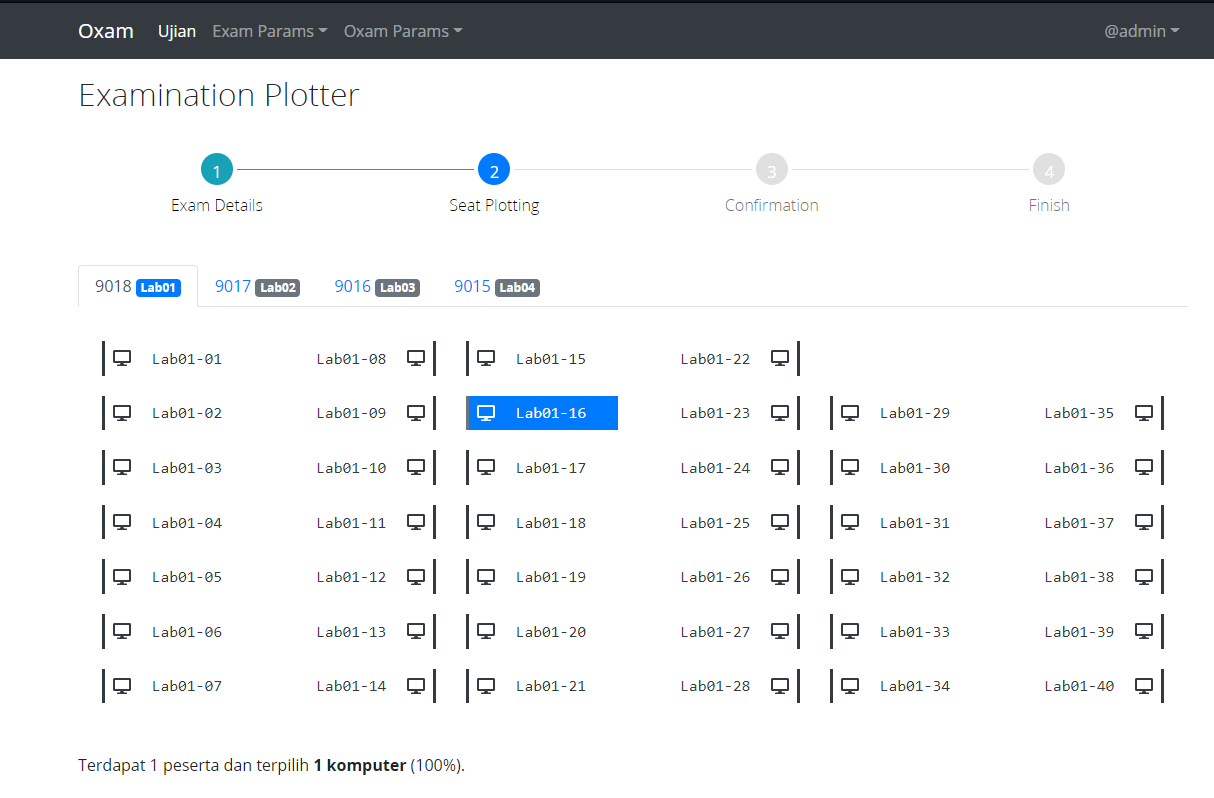
\includegraphics[width=0.8\textwidth]{images/seat-plotting.PNG}
    \caption{Pemilihan posisi duduk peserta ujian yang dilakukan secara manual.}
    \label{fig:seat-plotting}
\end{figure}

Gambar \ref{fig:seat-plotting} merupakan tampilan pada OXAM ketika Admin melakukan pemilihan posisi ujian peserta. Pemilihan posisi ujian dilakukan secara manual dengan cara memilih satu per satu komputer yang akan digunakan. Komputer-komputer yang sudah dipilih kemudian digunakan untuk menempatkan peserta ujian secara acak. OXAM kemudian akan menghasilkan \textit{script} berdasarkan hasil pemilihan acak tersebut. \textit{Script} yang dihasilkan nantinya akan dijalankan di \textit{server} untuk mendistribusikan berkas ujian. 

Berdasarkan ilustrasi di atas, terdapat beberapa usulan pengembangan pada mekanisme pemilihan posisi ujian. Usulan berfokus pada pencegahan terjadinya \textit{human error} pada saat pemilihan komputer yang dilakukan satu per satu yang sebenarnya dapat diotomatisasi berdasarkan jumlah peserta ujian. Selain itu, tampilan pada saat akan memilih posisi tidak menggambarkan kondisi komputer secara \textit{real time}. Pencatatan kondisi komputer dilakukan secara manual dan terpisah dari sistem. Hal ini mengakibatkan komputer yang dipilih mungkin saja berada dalam kondisi rusak, kosong tidak tersedia, memiliki masalah jaringan, atau masalah teknikal lainnya yang dapat mengakibatkan kendala pada saat pelaksanaan ujian. Dengan adanya pemeriksaan kondisi komputer secara \textit{real time} yang terintegrasi dengan sistem, masalah-masalah tersebut dapat terdeteksi lebih awal. Pemilihan secara acak pun dapat disesuaikan dengan ketersediaan komputer yang ada.

Kekurangan lainnya terkait dengan posisi komputer dan juga \textit{layout} tiap ruang lab ujian yang dibuat secara \textit{hardcode}. Jika terjadi perpindahan ruang lab yang mengakibatkan berubahnya layout ruangan, maka aplikasi menjadi tidak dapat digunakan. Pengembangan diharapkan dapat mempermudah penambahan atau pergantian \textit{layout} pada aplikasi OXAM yang dilakukan secara interaktif.

OXAM saat ini hanya dapat digunakan untuk menangani ujian yang dilakukan secara langsung di ruangan lab. Hal ini dikarenakan, otentikasi yang digunakan berdasarkan IP \textit{Address} dari komputer yang ada di ruangan lab. IP \textit{address} dari komputer yang melakukan akses ke \textit{endpoint} ujian akan dicocokan dengan kumpulan IP \textit{Address} komputer lab yang ada di \textit{database}. Jika IP \textit{Address} termasuk di dalam kumpulan IP \textit{Address} maka \textit{request} akan diproses lebih lanjut. Untuk mengatasi masalah ini, maka akan dibuat mode otentikasi berbasis token. Dengan adanya mode berbasis token, \textit{login} dapat dilakukan tanpa bergantung pada IP \textit{address} komputer serta peserta dapat mengikuti ujian dari luar ruangan lab. Dengan adanya mode berbasis token kegunaan OXAM dapat bertambah selain digunakan untuk UTS dan UAS, yakni digunakan pula untuk kuis maupun latihan. 

Pada skripsi ini akan dilakukan pengembangan pada OXAM dengan lebih berfokus pada pengembangan mekanisme pemilihan posisi ujian, pengaturan \textit{layout} yang dibuat agar lebih interaktif, dan penambahan mode berbasis token. 

\newpage

\section{Rumusan Masalah}
\label{sec:rumusan}

Berdasarkan deksripsi yang sudah dipaparkan di bagian \ref{sec:deskripsi}, terdapat beberapa hal yang menjadi poin utama untuk dijadikan sebagai rumusan masalah pada skripsi ini. Beberapa hal tersebut adalah:
\begin{enumerate}
    \item Bagaimana mekanisme yang diperlukan untuk menangani pemilihan posisi peserta ujian dengan tetap memperhatikan keadaan komputer secara \textit{real time} dan manajemen ruang pada laboratorium komputasi FTIS secara interaktif?
    \item Bagaimana mekanisme yang diperlukan untuk menerapkan mode otentikasi berbasis token dalam penggunaan OXAM?
    \item Bagaimana implementasi mode otentikasi berbasis token pada OXAM?
    \item Bagaimana implementasi untuk menghasilkan sistem yang dapat melakukan pemilihan posisi peserta ujian dengan tetap memperhatikan keadaan komputer secara \textit{real time} dan sistem manajemen ruang pada laboratorium komputasi FTIS secara interaktif?
\end{enumerate}

\section{Tujuan}

Berdasarkan bagian \ref{sec:deskripsi} dan bagian \ref{sec:rumusan}, dapat ditetapkan beberapa hal yang menjadi tujuan dari skripsi ini.

\begin{enumerate}
    %\item Mengetahui mekanisme penanganan manajemen ruang pada laboratorium komputasi FTIS secara interaktif dan pemilihan posisi peserta ujian dengan memperhatikan keadaan atau kondisi \textit{real time} dari komputer
    \item Menghasilkan spesifikasi kebutuhan dan rancangan untuk membuat sistem pemilihan posisi peserta ujian dengan memperhatikan keadaan atau kondisi \textit{real time} dari komputer dan sistem manajemen ruang pada laboratorium komputasi FTIS secara interaktif .
    \item Menghasilkan rancangan untuk menerapkan mode otentikasi berbasis token pada OXAM.
    \item Menghasilkan sistem pemilihan posisi ujian peserta secara acak dengan memperhatikan keadaan atau kondisi \textit{real time} dari komputer dan sistem manajemen ruang laboratorium komputasi FTIS yang dapat dilakukan secara interaktif menggunakan \textit{canvas} yang terintegrasi dengan OXAM.
    %\item Mengetahui mekanisme yang diperlukan untuk menerapkan mode berbasis token dalam penggunaan OXAM
    %\item Implementasi sistem manajemen ruang pada laboratorium komputasi FTIS yang interaktif dan pemilihan penempatan posisi peserta ujian yang memperhatikan keadaan komputer secara \textit{real time}
    %\item Implementasi sistem manajemen ruang pada laboratorium komputasi FTIS secara interaktif dan pemilihan penempatan posisi peserta ujian dengan memperhatikan keadaan komputer secara \textit{real time}
    %\item Implementasi mode berbasis token pada OXAM
    \item Menghasilkan mode ujian dengan otentikasi berbasis token pada OXAM yang dapat berjalan tanpa menggangu mode berbasis IP \textit{Address}.
\end{enumerate}


\section{Detail Perkembangan Pengerjaan Skripsi}
Detail bagian pekerjaan skripsi sesuai dengan rencana kerja/laporan perkembangan terakhir :
	\begin{enumerate}
		\item \textbf{Mempelajari cara kerja OXAM dan skripsi dari Gunawan Christianto (2016730011).}\\
		{\bf Status :} Ada sejak rencana kerja skripsi.\\
		{\bf Hasil :} Dilakukan dengan cara mempelajari arsitektur aplikasi yang digunakan pada OXAM v.5.0 yang dibuat oleh Gunawan Christianto. Studi dilakukan terhadap \textit{tools} yang digunakan, sistem, serta alur dari program OXAM.
		
% 		{\bf Hasil :} Dilakukan dengan cara mempelajari arsitektur aplikasi yang digunakan pada OXAM v.5.0 yang dibuat oleh Gunawan Christianto. Studi dilakukan terhadap \textit{tools} yang digunakan, sistem, desain ACL, penggunaan \textit{library} seperti JWT, serta alur dari program OXAM.
		
		\newpage
		\begin{itemize}
		    \item \textbf{Tools}\\
		    Terdapat beberapa \textit{tools} yang digunakan pada OXAM v.05, yaitu:
		    \begin{itemize}
		        \item \textbf{Docker}\\
		        \label{docker}
		        \textit{Docker} adalah sebuah \textit{platform containerization} yang bersifat \textit{open-source}.\footnote{Sumber berasal dari : \url{https://www.ibm.com/topics/docker}. Diakses pada 15 Desember 2021.} \textit{Containerization} adalah pengemasan kode perangkat lunak dengan \textit{library} dan dependensi sistem operasi (OS) yang diperlukan untuk menjalankan kode untuk membuat satu \textit{executable lightweight}—disebut \textit{container}—yang berjalan secara konsisten di infrastruktur apa pun. Lebih portabel dan hemat sumber daya daripada mesin virtual (VM), container telah menjadi unit komputasi \textit{de facto} dari aplikasi \textit{cloud-native} modern.\footnote{Sumber berasal dari: \url{https://www.ibm.com/topics/containerization}. Diakses pada 15 Desember 2021.}
		
        		\setlength\parindent{24pt}
        		Dengan adanya \textit{containerization}, \textit{developer} dapat membuat dan melakukan \textit{deploy} aplikasi secara cepat dan aman. Pada penggunaan metode tradisional, kode dikembangkan dalam lingkungan komputasi tertentu dan ketika dipindahkan ke lokasi baru sering mengakibatkan \textit{bug} dan kesalahan. Misalnya, ketika pengembang melakukan transfer kode dari komputer \textit{desktop} ke mesin virtual (VM) atau dari Linux ke sistem operasi Windows. \textit{Containerization} mengeliminasi masalah ini dengan menggabungkan kode aplikasi bersama dengan \textit{file} konfigurasi terkait, \textit{library}, dan dependensi yang diperlukan untuk menjalankannya. Paket perangkat lunak atau "wadah" tunggal ini diabstraksikan dari sistem operasi \textit{host}, sehingga dapat berdiri sendiri dan menjadi portabel—dapat dijalankan di platform atau \textit{cloud} apa pun, bebas dari masalah.\footnote{Ibid.}
        		
        		Selain terkait dengan portabilitas dari \textit{container}, \textit{resource} seperti memori yang digunakan oleh \textit{container} cenderung lebih ringan. Hal ini dikarenakan alokasi diberikan sesuai dengan kebutuhan container. Berbeda dengan VM yang memorinya dialokasikan dengan ukuran tertentu sejak awal dan kemudian dikunci, sehingga kelebihan alokasi menjadi tidak terpakai.
        		
                Integrasi dari perubahan pada \textit{image} yang digunakan oleh \textit{container} pun terbilang lebih mudah, karena perubahan cukup dilakukan pada file konfigurasi yang digunakan untuk membuat \textit{image}. \textit{Developer} tidak lagi harus melakukan penambahan secara manual, karena sudah dilakukan secara otomatis oleh \textit{docker}. Docker juga mendukung penggunaan CI/CD yang memungkinkan untuk dilakukan \textit{tracking} pada versi \textit{image} yang dirubah.
                
                	\begin{figure}[H]
                    \centering
                    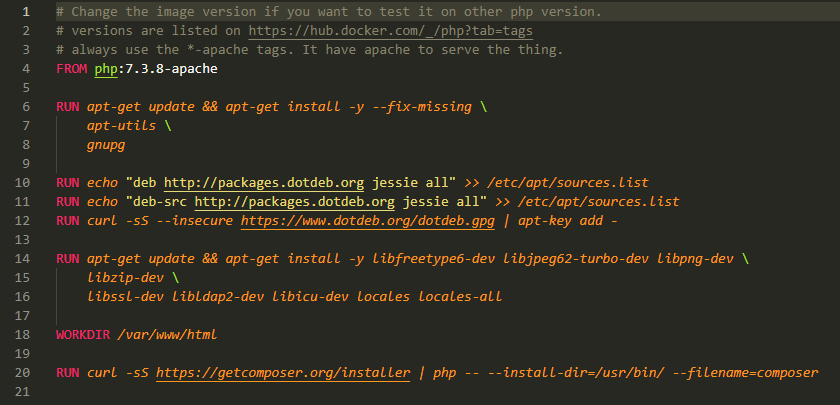
\includegraphics[width=0.75\textwidth]{images/dockerfile.PNG}
                    \caption{Isi dari Dockerfile yang digunakan pada aplikasi OXAM. Menggunakan \textit{base image} php:7.3.8-apache yang berisi Apache httpd Debian. Terdapat instruksi-instruksi yang digunakan untuk membuat \textit{image}. Sebagai contoh, instruksi untuk melakukan \textit{download package} tambahan yang dibutuhkan untuk Debian dari \textit{repository} dotdeb.org dan sebagainya.}
                    \label{fig:dockerfile}
                \end{figure}
                
                \textit{Docker} menggunakan file konfigurasi yang diberi nama Dockerfile untuk membangun \textit{image} yang dibutuhkan untuk membuat \textit{container}. File konfigurasi ini berisi, \textit{base image} yang akan digunakan serta runtutan instruksi yang dibutuhkan untuk membuat lingkungan yang dapat digunakan untuk menjalankan aplikasi secara lancar. Contoh dari Dockerfile yang digunakan pada aplikasi OXAM dapat dilihat di Gambar \ref{fig:dockerfile}.
                
                Selain Dockerfile, terdapat file konfigurasi lain bernama docker-compose.yml yang digunakan untuk menjalankan lebih dari satu kontainer sebagai sebuah service. Tiap container berjalan secara terisolasi, namun tetap dapat berinteraksi satu sama lain ketika dibutuhkan. Pada file ini, dapat ditentukan jenis-jenis \textit{service} yang akan dijalankan, volume yang digunakan oleh \textit{service}, \textit{port} yang digunakan untuk menghubungkan \textit{host} dengan \textit{container}, dan konfigurasi-konfigurasi lainnya yang dibutuhkan oleh \textit{service}.
                \\
                \\
        	\item \textbf{Gitlab \textit{Continuous Integration/Continuous Delivery/Deployment} (CI/CD)}\\
		        \label{gitlab-cicd}
                Gitlab CI/CD adalah \textit{tool} pengembangan perangkat lunak yang menggunakan metodologi berkelanjutan.\footnote{Sumber berasal dari: \url{https://docs.gitlab.com/ee/ci/}. Diakses pada 16 Desember 2021.} Terdapat tiga bagian utama dari CI/CD, yaitu:
        		\begin{itemize}
        		    \item \textit{ Continuous Integration}, dilakukan dengan cara memanfaatkan \textit{script} untuk membangun dan melakukan uji coba pada aplikasi secara otomatis terhadap perubahan yang dilakukan oleh \textit{developer}.
        		    \item \textit{ Continuous Delivery}, berada selangkah setelah \textit{ Continuous Integration}. Selain melakukan uji coba, juga dilakukan \textit{deploy} secara manual terhadap perubahan yang ada secara berkelanjutan.
        		    \item \textit{ Continuous Deployment}, memiliki kemiripan dengan \textit{ Continuous Delivery}, namun \textit{deploy} dari perubahan dilakukan secara otomatis. \footnote{Sumber berasal dari: \url{https://docs.gitlab.com/ee/ci/introduction/index.html\#continuous-integration}. Diakses pada 16 Desember 2021.}
        		\end{itemize}
        		
        		\begin{figure}[H]
                    \centering
                    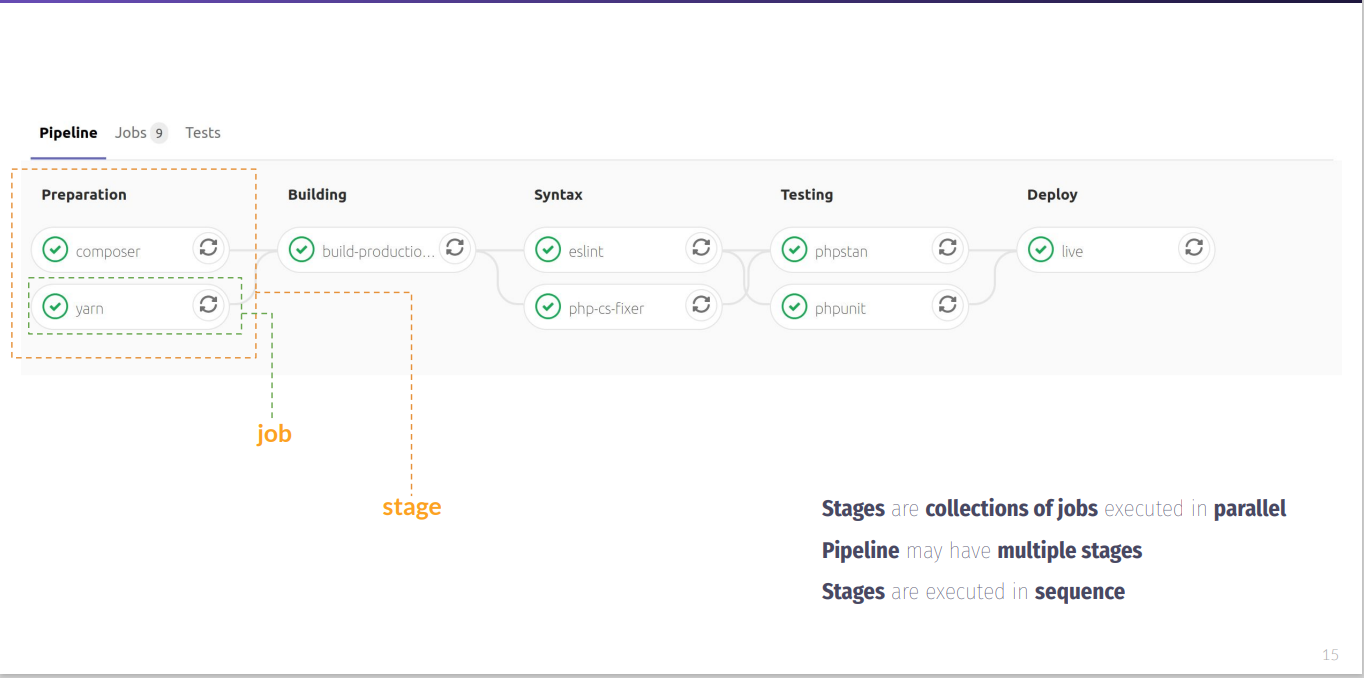
\includegraphics[width=0.85\textwidth]{images/gitlab-ci-cd.PNG}
                    \caption{Pada ilustrasi ini dapat dilihat, bagian terkecil di dalam sebuah \textit{pipeline} adalah sebuah \textit{job}. \textit{Jobs} yang tersusun atau dijalankan secara paralel membentuk \textit{stage}. Lalu kumpulan \textit{stage} yang dieksekusi secara berurutan kemudian menjadi sebuah \textit{pipeline}.}
                    \label{fig:gitlab-concepts}
                \end{figure}
        		
                 Terdapat beberapa istilah dasar terkait dengan penggunaan CI/CD, yaitu:
                 \begin{itemize}
                     \item \textit{Pipeline} yang merupakan kumpulan dari satu atau lebih \textit{job}. Dapat dibagi menjadi kumpulan \textit{stage}
                     \item \textit{Stages} merupakan kumpulan \textit{job} yang dijalankan secara paralel. Beberapa contoh \textit{stage} yang umum digunakan, \textit{Build}, \textit{Test}, \textit{Deploy}, dan sebagainya
                     \item \textit{Jobs} dapat berupa \textit{script} yang menjalankan tugas tertentu
                 \end{itemize}
                 
                 \begin{figure}[H]
                    \centering
                    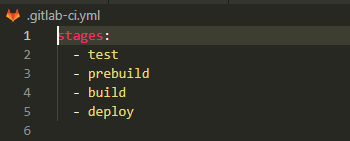
\includegraphics[width=0.65\textwidth]{images/gitlab-stages.PNG}
                    \caption{Beberapa \textit{stage} yang ada pada CI/CD yang digunakan oleh OXAM}
                    \label{fig:gitlab-stages}
                \end{figure}
        		
                 Konfigurasi CI/CD dilakukan dengan cara menyertakan \textit{file} .gitlab-ci.yml pada direktori \textit{root} dari aplikasi. Umumnya diawali dengan melakukan deskripsi dari \textit{stage} yang ada pada pipeline. Contoh dari pendeskripsian \textit{stage} pada \textit{file}  .gitlab-ci.yml dapat dilihat pada Gambar \ref{fig:gitlab-stages}. \textit{Stage} ini kemudian nantinya akan direferensikan pada job yang dideskripsikan. 
                 
                 
                 	\begin{figure}[H]
                    \centering
                    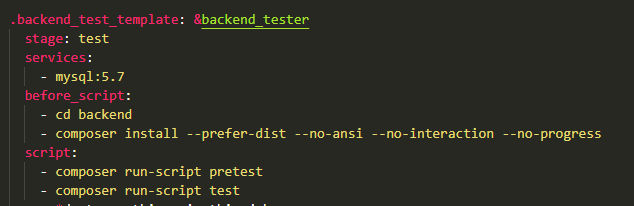
\includegraphics[width=0.65\textwidth]{images/gitlab-job-test-backend-temp.PNG}
                    \caption{Berikut merupakan \textit{job} backend\_test\_template yang masuk ke dalam \textit{stage} \textit{Test}.}
                    \label{fig:gitlab-job-test-backend-temp}
                \end{figure}
        		
                 Seperti yang terlihat pada Gambar \ref{fig:gitlab-job-test-backend-temp}, terdapat \textit{before\_script} dan \textit{script} yang merupakan sebuah \textit{task} yang akan dilakukan pada sebuah job. Terdapat beberapa jenis eksekusi \textit{script}, yaitu:
                 \begin{itemize}
                     \item before\_script: dijalankan terlebih dahulu sebelum perintah yang ada pada \textit{script} dijalankan
                     \item after\_script: dijalankan ketika keseluruhan \textit{job} selesai 
                 \end{itemize}
                 
                 Selain \textit{script}, dapat disertakan pula jenis \textit{service} yang digunakan pada sebuah \textit{job}. Seperti yang terlihat pada Gambar \ref{fig:gitlab-job-test-backend-temp}, \textit{service} yang digunakan untuk \textit{job} tersebut adalah \textit{service} basis data yang menggunakan mysql versi 5.7. Selain mencatumkan jenis \textit{service} dapat pula dicantumkan jenis \textit{image} yang digunakan untuk menjalankan sebuah \textit{job}. \textit{Image} yang dicantumkan akan digunakan oleh \textit{Docker executor} untuk menjalankan \textit{job} yang bersangkutan.
                 
                 Jika dilihat kembali, pada Gambar \ref{fig:gitlab-job-test-backend-temp} \textit{job} backend\_test\_template diawali dengan tanda titik. Tanda ini digunakan untuk menandai sebuah \textit{job} sebagai \textit{hidden job}, sehingga tidak langsung dieksekusi. Job ini akan dieksekusi apabila diikutsertakan ke job lainnya dengan melakukan referensi ke \textit{anchor} yang dimiliki oleh \textit{hidden job}. Pada Gambar \ref{fig:gitlab-job-test-backend-temp}, \textit{anchor} untuk \textit{job} tersebut didefinisikan setelah tanda titik dua (:) dengan menambahkan tanda \textit{ampersand} (\&) sebelum nama dari \textit{anchor} sesuai yang terlihat pada Gambar \ref{fig:gitlab-job-test-backend} (``\&backend\_tester'').
                 
                 \begin{figure}[H]
                    \centering
                    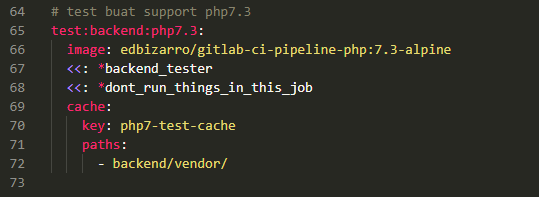
\includegraphics[width=0.65\textwidth]{images/gitlab-job-test-backend.PNG}
                    \caption{Berikut merupakan \textit{job} test:backend yang masuk ke dalam \textit{stage} \textit{Test}.}
                    \label{fig:gitlab-job-test-backend}
                \end{figure}
        		
        		Pada \textit{job} test:backend yang dapat dilihat pada Gambar \ref{fig:gitlab-job-test-backend}, \textit{job}  backend\_test\_template diikutsertakan dengan cara mereferensikan \textit{hidden job}. Untuk mereferensikan \textit{hidden job} digunakan tanda \textit{asterisk} diikuti dengan nama dari \textit{anchor}. Tanda ``<<'' digunakan untuk melakukan \textit{merge} isi dari \textit{anchor} ``backend\_tester''. 
		    \end{itemize}
		    % End of tools section
		    \vspace{0.5cm}
		    \item \textbf{Sistem yang digunakan oleh OXAM}\\
		    \label{sectionsystem}
		    
    		OXAM terdiri dari 2 buah subsistem, yang dirancang menggunakan library yang berbeda, yaitu:
    		
    		\begin{itemize}
    		    \item \textbf{Backend}\\
    		    \label{backend}
    		    \textit{Back-end} merupakan subsistem dari sebuah aplikasi \textit{web} yang tidak terlihat dan tidak terhubung secara langsung dengan \textit{client}. \textit{Back-end} menjadi perantara yang menghubungkan infrastruktur seperti basis data dengan bagian \textit{front-end} yang menangani \textit{client}. Tugas dari \textit{back-end} sendiri cukup bervariasi, seperti menangani \textit{request} halaman \textit{web}, melakukan pengolahan data baik untuk disimpan ataupun diperbaharui di basis data, menangani \textit{upload} maupun \textit{download} dari \textit{file}, dan masih banyak lagi. 
    		
        		Proses data yang dilakukan oleh \textit{back-end} dilakukan di sisi server. Umumnya \textit{client} tidak akan menyadari ada subsistem ini, karena interaksi dilakukan hanya dengan \textit{front-end}. Pada OXAM v.5.0, subsistem ini diimplementasikan menggunakan \textit{framework} FatFree dan menggunakan arsitektur REST.
    		    
    		    \item \textbf{Frontend}\\
    		    \label{frontend}
    		    Berbeda dengan \textit{back-end}, \textit{front-end} merupakan subsistem yang berinteraksi secara langsung dengan \textit{client}. Tugas dari \textit{front-end} sendiri adalah untuk menampilkan data secara interaktif dan menarik kepada \textit{client}, menangani input yang diberikan oleh \textit{client} sesuai alur tertentu kemudian diteruskan ke \textit{back-end} untuk diproses lebih lanjut. Karena terletak di sisi \textit{client}, subsistem ini tidak menutup kemungkinan untuk dimanfaatkan sebagai celah untuk menyerang \textit{server}. Sanitasi input yang diberikan dari bagian \textit{front-end} ke \textit{back-end} perlu dilakukan untuk mencegah sistem mengalami hal yang tidak diinginkan. Pada OXAM v.5.0, subsistem \textit{front-end} diimplementasikan menggunakan \textit{library} React.js.
    		    
    		\end{itemize}
		
% 		\item \textbf{Desain \textit{Access Control List} (ACL)}
% 		\label{sectionacl}
		
		
% 		\item \textbf{Penggunaan JWT untuk melakukan Otentikasi}
% 		\label{sectionjwt}
		  %  End of system section
		    
		\end{itemize}
		
		
		\item \textbf{Mempelajari React.js sebagai \textit{library front-end}.}\\
		{\bf Status :} Ada sejak rencana kerja skripsi.\\
		{\bf Hasil :} React.js merupakan \textit{library} Javascript yang  digunakan membuat \textit{user interface}.\footnote{\url{https://reactjs.org/}. Diakses pada 31 Desember 2021} Terdapat beberapa kelebihan yang dimiliki oleh \textit{library} ini sehingga menjadi  salah satu \textit{library} yang banyak digunakan saat ini. Salah satu kelebihan dari React.js adalah sifatnya yang deklaratif. Pemrograman deklaratif berfokus untuk membangun \textit{logic} dari program tanpa benar-benar mendeskripsikan alur yang dibutuhkan. React.js memiliki bentuk yang mirip dengan HTML. Bentuk deklaratif pada HTML sebagai contoh adalah ketika mendeklarasikan elemen \texttt{<img src=`./image.jpg' />} agar browser menampilkan sebuah gambar. Proses atau \textit{flow} agar gambar tersebut tampil di browser tidak menjadi fokus utama. Fokus utama yang ingin dicapai adalah ``apa'', dalam hal ini sebuah gambar dengan \textit{source} asal gambar image.jpg.
		
		Sifat lain dari React.js adalah berbasis komponen. Pengguna dapat mendeklarasikan komponen dengan \textit{state} tersendiri, kemudian membentuk komponen tersebut menjadi sebuah UI yang kompleks. Selain itu, React.js memungkinkan pengguna untuk ``Pelajari sekali, tulis dimanapun" atau disebut juga ``\textit{Learn once, write anywhere}'' (LOWA).\footnote{\url{https://reactjs.org/}. Diakses pada 31 Desember 2021}
		\\
		\\
		\setlength\parindent{0pt}
		\textbf{Javascript XML (JSX)}\\
		React.js menggunakan sintaks Javascript XML atau disingkat JSX. Javascript XML merupakan turunan dari Javascript yang memungkinkan penggunaan HTML dalam Javascript. Untuk mendeklarasikan sebuah komponen React menggunakan sintaks JSX, pengguna dapat membuat elemen dalam bentuk yang mirip dengan elemen pada HTML. Sebuah elemen memiliki \textit{tag} buka dan juga \textit{tag} penutup. Sebuah \textit{tag} diawali dengan tanda ``<'' dan diakhiri dengan tanda ``>''. Untuk \textit{tag} penutup setelah diawali dengan tanda ``<'' diikuti dengan tanda \textit{slash} (/) lalu diakhiri dengan tanda ``>''.
		
		\begin{figure}[H]
            \centering
            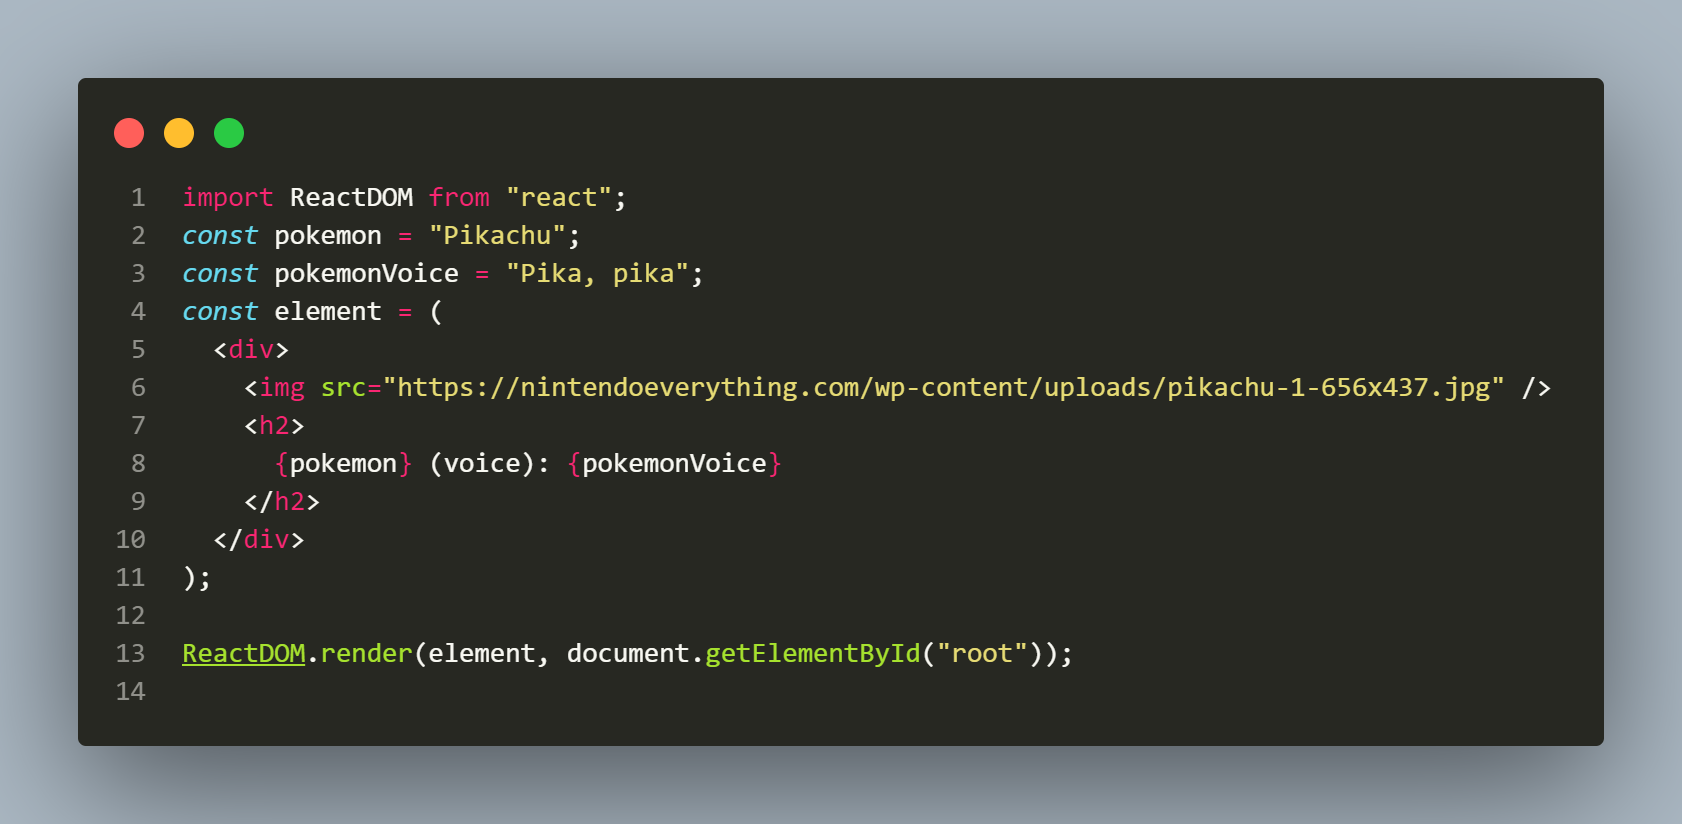
\includegraphics[width=0.8\textwidth]{images/code-jsx.png}
            \caption{Potongan kode yang menunjukan penggunaan elemen HTML pada Javascript}
            \label{fig:react-code-jsx}
        \end{figure}
		
		\setlength\parindent{24pt}
		Gambar \ref{fig:react-code-jsx} merupakan contoh potongan kode JSX, yang menggunakan elemen HTML \textit{Heading 2} untuk mengeluarkan sebuah gambar diikuti dengan potongan teks \texttt{Pikachu (voice): Pika, pika} yang akan di\textit{render} ke elemen HTML dengan id \textit{root}. Penggunaan elemen HTML yang memerlukan atribut tertentu tetap dimungkinkan dalam penggunaan JSX. Seperti yang terlihat pada Gambar \ref{fig:react-code-jsx}, penggunaan elemen HTML \textit{img} yang memerlukan atribut \textit{src} akan di\textit{render} secara normal.
		\\
		\\
		\setlength\parindent{0pt}
		\textbf{Komponen pada React}\\
		Pada React.js terdapat 2 cara untuk membuat komponen React, yaitu dengan mendeklarasikan komponen sebagai sebuah \textit{class} dan menjadikan \textit{class} tersebut turunan dari React.Component (\textit{class component}) atau dengan mendeklarasikannya sebagai sebuah fungsi (\textit{function component}). 
		
		\begin{figure}[H]
            \centering
            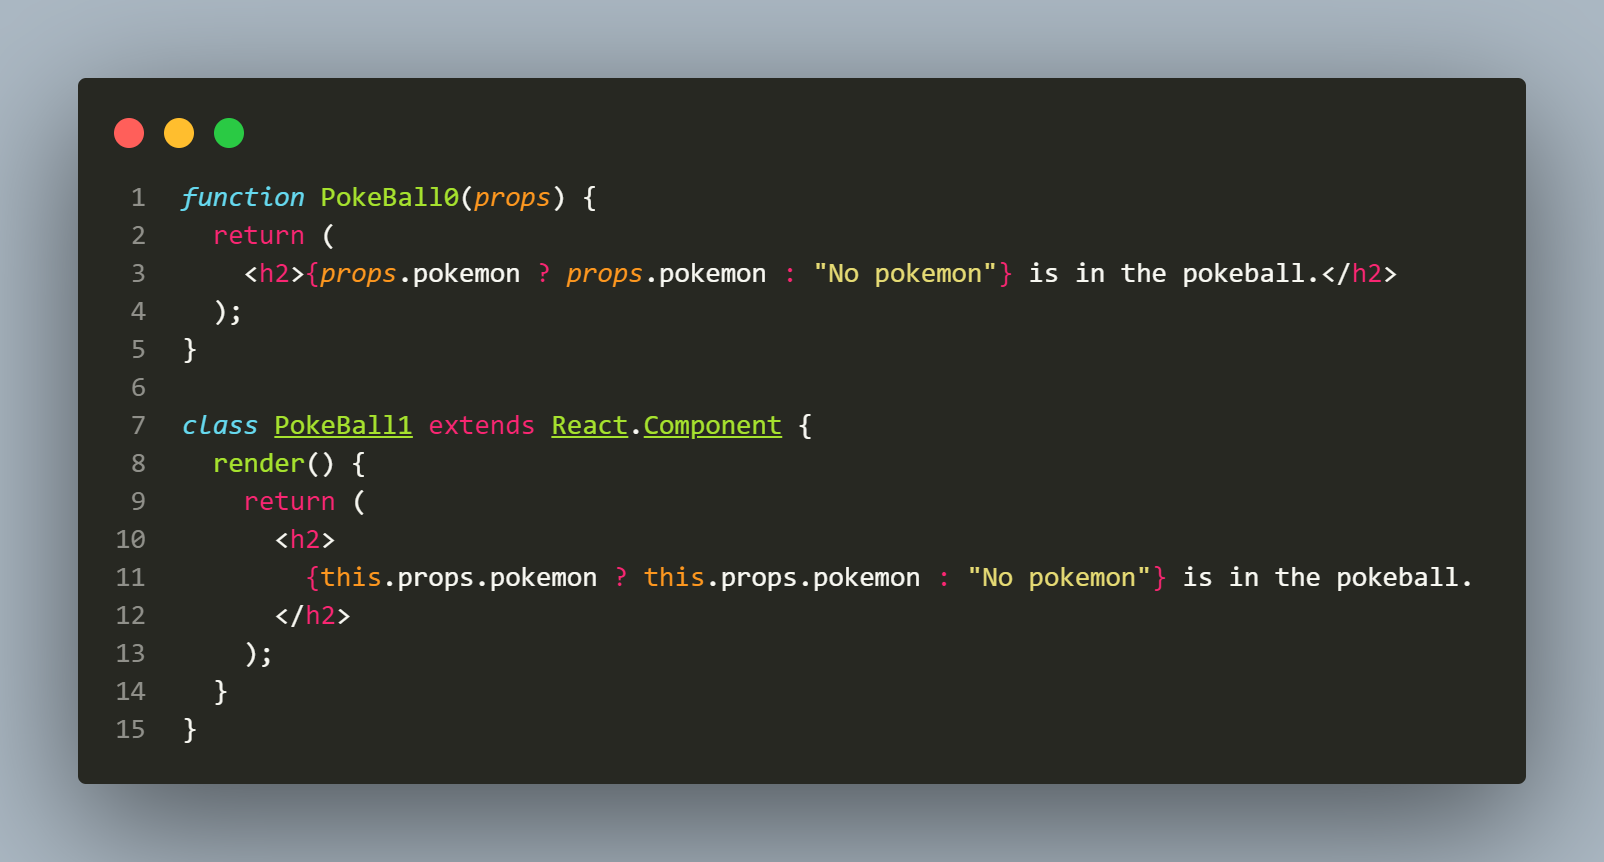
\includegraphics[width=0.8\textwidth]{images/code-class-func-comp.png}
            \caption{Potongan kode yang menunjukan deklarasi \textit{functional component} \texttt{Pokeball0} dan \textit{class component} \texttt{Pokeball1}.}
            \label{fig:react-code-class-func-comp}
        \end{figure}
		\setlength\parindent{24pt}
		Jika dilihat pada Gambar \ref{fig:react-code-class-func-comp}, \textit{functional component} memiliki cara deklarasi komponen yang lebih \textit{simple} dibandingkan dengan \textit{class component}. Kedua komponen sama-sama menerima input masukan melalui \texttt{props} sebagai parameter pada \textit{functional component} dan sebagai atribut pada \textit{class component}.
		\\
		\\
		\setlength\parindent{0pt}
		\textbf{\textit{State} pada React}\\
		Pada Gambar \ref{fig:react-code-class-func-comp} terlihat input untuk komponen dimasukkan melalui \texttt{props}. \texttt{Props} (singkatan dari \textit{properties}) dan \texttt{state} merupakan objek pada Javascript. Keduanya menyimpan informasi yang mempengaruhi \textit{output} hasil \textit{render}, namun memiliki perbedaan yang cukup penting untuk diperhatikan; \texttt{props} dimasukkan sebagai input ke komponen (sama seperti parameter pada fungsi), sedangkan \texttt{state} dikelola di dalam komponen (mirip dengan variabel yang dideklarasikan dalam suatu fungsi).\footnote{\url{https://reactjs.org/docs/faq-state.html}. Diakses pada 31 Desember 2021}\\
		
		\setlength\parindent{24pt}
		\texttt{Props} memiliki sifat yang \textit{immutable} atau tidak dapat diubah-ubah. Berbeda dengan \texttt{state} yang merupakan \textit{observable object} yang menyimpan data yang nilainya dapat berubah sewaktu-waktu. Karena dikelola di dalam komponen, \texttt{state} dapat digunakan untuk mengontrol perilaku (\textit{behavior}) dari komponen. Perubahan pada \texttt{state} mengakibatkan \textit{render} ulang dilakukan pada komponen. 
		
		Sebelum adanya React versi 16.8, penggunaan \texttt{state} tidak dimungkinkan pada \textit{functional component}. Penggunaan \texttt{state} hanya dimungkinkan dengan mendeklarasikan \textit{class component}. Pada versi 16.8, \texttt{state} dan fitur lainnya pada React dapat digunakan tanpa perlu mendeklarasikan \textit{class component} (menggunakan \textit{functional component}). Pada \textit{class component} state masih dikelola sebagai atribut, sedangkan pada \textit{functional componen} \texttt{state} dikelola menggunakan \textit{hook}. \textit{Hook} merupakan fungsi spesial pada React yang memungkinkan untuk menghubungkan fungsi ke fitur React. \textit{Hook} hanya dapat digunakan pada \textit{functional component}.\footnote{\url{https://reactjs.org/docs/hooks-state.html}}
		
		
		\begin{figure}[H]
            \centering
            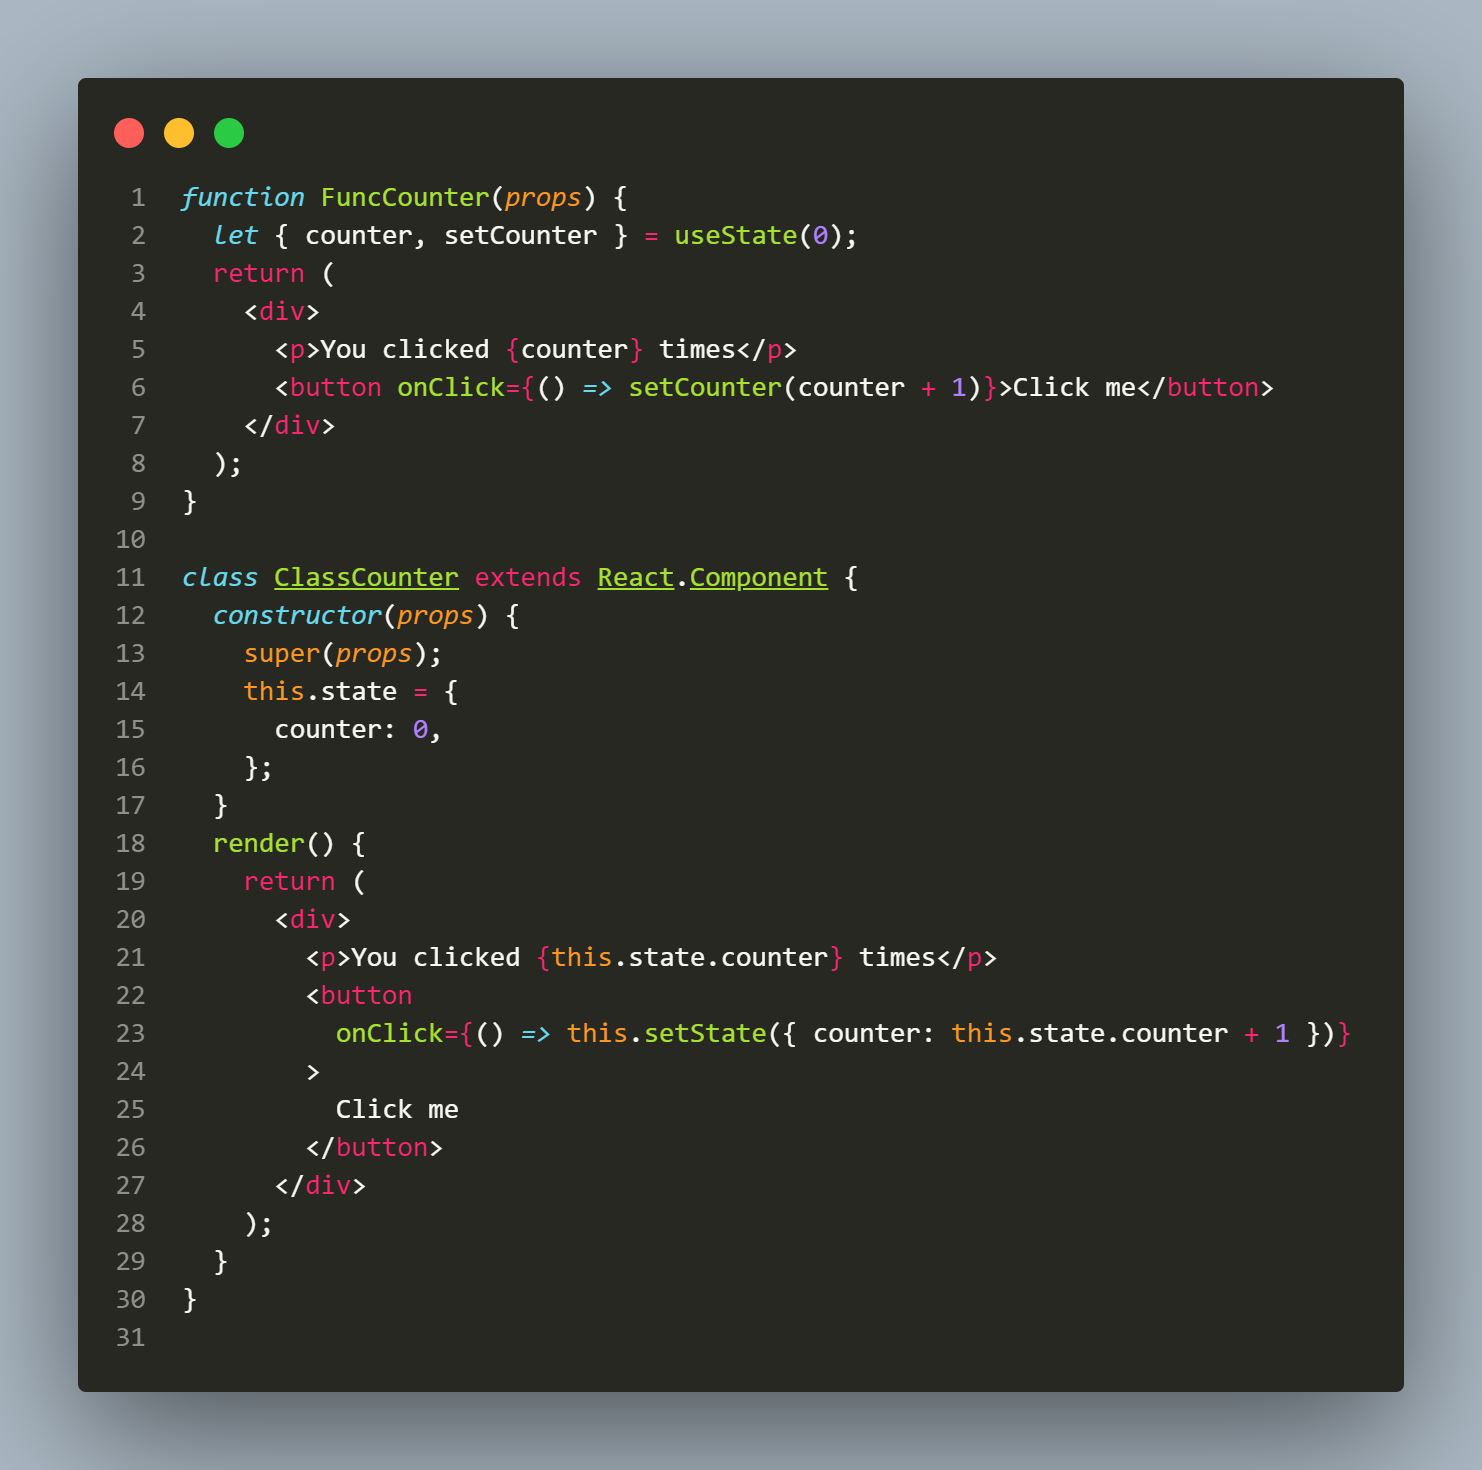
\includegraphics[width=0.7\textwidth]{images/code-class-func-state.png}
            \caption{Potongan kode yang menunjukan deklarasi \textit{functional component} \texttt{Pokeball0} dan \textit{class component} \texttt{Pokeball1}.}
            \label{fig:react-code-class-func-state}
        \end{figure}
        
        Gambar \ref{fig:react-code-class-func-state} menunjukan pengelolaan \texttt{state} pada \textit{functional component} dan \textit{class component}. Kedua komponen akan melakukan \textit{render} sebuah tombol dan juga teks yang akan menampilkan jumlah aksi tekan yang sudah dilakukan pada tombol. Setiap kali tombol ditekan, kedua komponen akan melakukan \textit{render} ulang dengan nilai \texttt{counter} yang sudah diperbaharui. \textit{Hook} \texttt{useState} digunakan untuk mengelola \texttt{state} pada \textit{functional component}.
        
		\item \textbf{Mempelajari FatFree  sebagai \textit{framework} yang digunakan untuk \textit{back-end}.}\\
		{\bf Status :} Ada sejak rencana kerja skripsi.\\
		{\bf Hasil :} Fatfree merupakan \textit{micro-framework} yang \textit{powerful} namun mudah digunakan untuk membangun aplikasi \textit{web} yang dinamis.\footnote{\url{https://github.com/bcosca/fatfree}. Diakses pada 20 Desember 2021.} Fatfree sesuai dengan yang diimplikasikan oleh namanya \textit{fat free} memiliki ukuran yang terbilang cukup kecil (diringkas dalam satu \textit{file} berukuran \~65KB) memungkinkan \textit{developer} untuk menciptakan aplikasi \textit{web} dengan eksekusi yang lebih cepat.\\
		Fatfree merupakan salah satu \textit{framework} dengan dokumentasi yang sangat baik. Selain itu \textit{effort} yang diperlukan untuk mempelajari framework ini hampir tidak ada. FatFree memberikan kebebasan untuk menyelesaikan lebih banyak pekerjaan dengan waktu yang lebih sedikit. \footnote{\url{https://fatfreeframework.com/3.7/getting-started}. Diakses pada 20 Desember 2021.} Penggunaan \textit{composer} bersamaan dengan Fatfree mendukung pengelolaan \textit{package} yang lebih terpusat. Dengan menambahkan Fatfree sebagai \textit{dependencies} pada \textit{file} composer.json dan memanggil perintah \textit{composer install}, \textit{package} yang dibutuhkan terkait dengan Fatfree akan diunduh secara otomatis.\\
		\\
		\newpage
		\setlength\parindent{0pt}
		\textbf{Hello World from Fatfree}
		\setlength\parindent{24pt}
		 \begin{figure}[H]
            \centering
            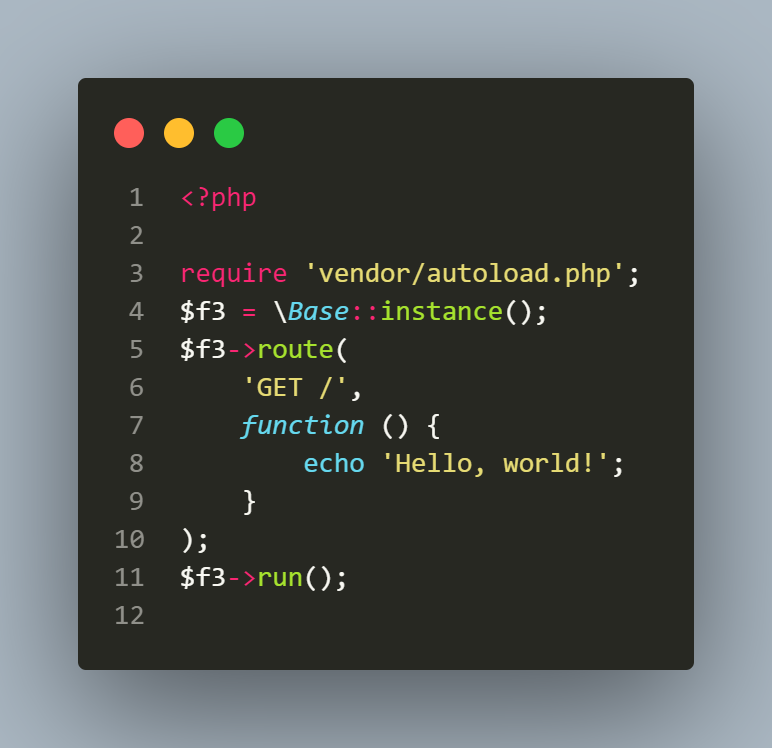
\includegraphics[width=0.45\textwidth]{images/hello-world.png}
            \caption{Potongan kode \textit{Hello World} menggunakan Fatfree. Penggunaan bersamaan dengan \textit{composer} memudahkan \textit{include} \textit{file} yang dibutuhkan oleh sebuah proyek cukup dengan hanya mengikutsertakan \textit{file} autoload.php}
            \label{fig:f3-hello-world}
        \end{figure}
		
		Potongan kode pada Gambar \ref{fig:f3-hello-world}, dilakukan definisi sebuah halaman yang dapat diakses melalui URL \textit{slash} (/). Ketika \textit{client} melakukan akses ke halaman yang terletak pada \url{http://127.0.0.1/} akan ditampilkan tulisan ``Hello, world!''. Contoh pada Gambar \ref{fig:f3-hello-world}, merupakan \textit{route} yang akan menangani \textit{request} menggunakan metode HTTP GET. Metode HTTP \textit{request} lainnya dapat diimplementasikan dengan menyesuaikan parameter yang diberikan pada bagian \$f3->router().
		
		\textit{Request} ke sebuah \textit{path} dapat ditangani dengan menyertakan fungsi yang menjadi \textit{handler} seperti yang dapat dilihat pada Gambar \ref{fig:f3-hello-world}. Penerapan dengan cara ini dapat mengacaukan \textit{namespace} \textit{global} dengan nama fungsi. Fatfree memungkinkan \textit{developer} untuk melakukan \textit{mapping} routing antara sebuah \textit{path} dengan Kelas OOP dan juga method yang menjadi handler. 
		
			 \begin{figure}[H]
            \centering
            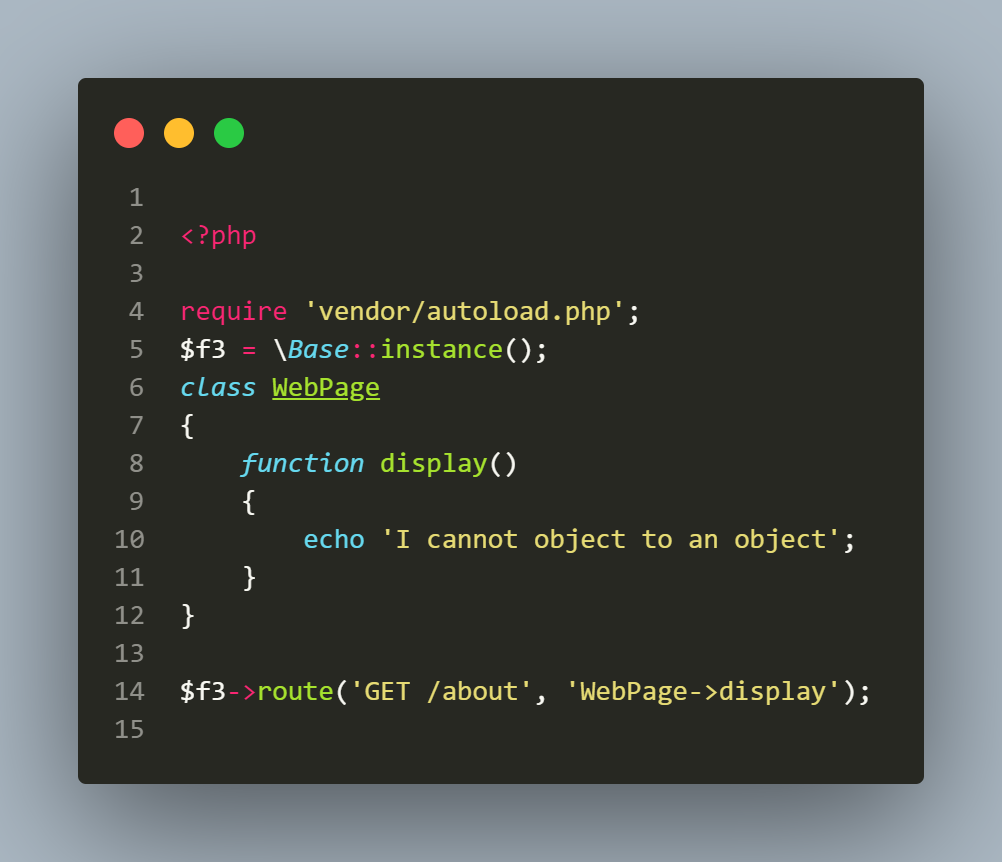
\includegraphics[width=0.45\textwidth]{images/hello-world-oop.png}
            \caption{\textit{Mapping} antara sebuah \textit{path /about} dengan kelas WebPage dengan \textit{method} display() sebagai \textit{handler}.}
            \label{fig:f3-hello-world-oop}
        \end{figure}
        
        Penggunaan mapping seperti pada Gambar \ref{fig:f3-hello-world-oop} memungkinkan desain kelas yang lebih seragam. Selain itu, perubahan pada fungsi dilakukan pada kelas yang bersangkutan, tidak bertebaran dan memudahkan \textit{developer} untuk melakukan \textit{maintain} pada kode.  
        
        
		\begin{figure}[H]
            \centering
            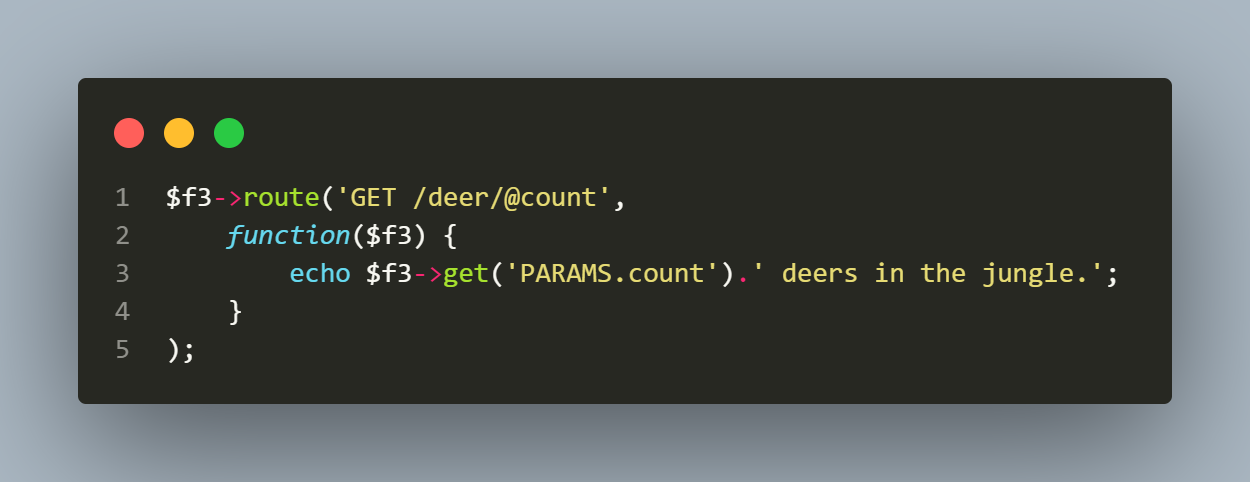
\includegraphics[width=0.75\textwidth]{images/route-beer-param.png}
            \caption{Token @count yang disertakan sebagai parameter pada URL \textit{request}.}
            \label{fig:route-beer-param}
        \end{figure}
        
        Seperti yang dapat dilihat pada Gambar \ref{fig:route-beer-param}, token dapat disertakan sebagai bagian dari sebuah URL. Token ini dapat diakses melalui \textit{global array} PARAMS pada variabel \$f3. Ketika \textit{client} melakukan \textit{request} ke URL \url{http://127.0.0.1/deer/8} akan dikembalikan keluaran ``8 \textit{deers in the jungle}''. Ketika \textit{client} melakukan \textit{request} ke URL \url{http://127.0.0.1/deer/majestic} akan~dikembalikan~keluaran `` \textit{majestic deers in the jungle}''.
        
		\item \textbf{Mengumpulkan kebutuhan dan melakukan analisis dampak.}\\
		{\bf Status :} Ada sejak rencana kerja skripsi.\\
		{\bf Hasil :}Pada bagian ini, kebutuhan untuk penelitian dikumpulkan dengan melihat kendala yang ada pada OXAM versi 5.0 dan juga fitur-fitur yang dapat dikembangkan berdasarkan usulan yang sudah dibahas pada bagian \ref{sec:deskripsi}.
		
		\begin{itemize}
		    \item \textbf{Kebutuhan dan Analisis Dampak}\\
		    \label{kebutuhan_analisis-dampak}
		     \begin{itemize}
		         \item \textbf{Kebutuhan}\\
		         \label{kebutuhan}
		         \setlength\parindent{0pt}
		         Berdasarkan penjabaran yang ada pada bagian \ref{sec:deskripsi}, terdapat beberapa hal yang dapat~diperbaiki dan fitur yang dapat ditambahkan pada OXAM v.5.0. Beberapa hal tersebut diantaranya adalah sebagai berikut:
		
            		\begin{enumerate}
            		    \item Manajemen ruang lab pada aplikasi OXAM yang dapat dibuat menjadi interaktif agar dapat menyesuaikan dengan perubahan layout ruangan.
            		    \item Pemilihan posisi ujian yang dapat diotomatisasi, sehingga tidak perlu sepenuhnya dilakukan secara manual oleh Tim Admin.
            		    \item Status komputer pada ruang lab dan aplikasi OXAM yang tidak sinkron/terintegrasi secara \textit{real time}.
            		    \item Penambahan mode ujian dengan otentikasi berbasi token yang mendukung pelaksanaan ujian dari luar ruangan lab.
            		    \item Pemindahan posisi ujian peserta (\textit{migrator}) yang disesuaikan dengan sistem manajemen ruang lab yang akan dibuat.
            		\end{enumerate}
            		
            		\vspace{0.3cm}
            		
            		\item \textbf{Manajemen Ruang dan Komputer}\\
            		\label{manajemen-ruang}
            		\setlength\parindent{0pt}
            		Pada aplikasi OXAM v.5.0, pemetaan ruang lab dan komputer yang ada masih dilakukan secara \textit{hardcode}. Data mengenai ruangan lab yang ada saat ini disimpan dengan memetakan secara manual. Sehingga apabila terjadi perubahan kedepannya terhadap \textit{layout} dari ruang lab, maka aplikasi OXAM tidak dapat digunakan. Usulan yang diberikan adalah untuk membuat sebuah sistem manajemen ruang lab yang dapat digunakan untuk melakukan penambahan ruang lab, perubahan, dan penyimpanan yang dilakukan secara interaktif.
		
		            \setlength\parindent{24pt}
            		Kebutuhan untuk melakukan manajemen ruang ini secara spesifik dikhususkan untuk Tim Admin. Beberapa fitur yang minimal tersedia pada sistem ini setelah didiskusikan dengan Dosen Pembimbing adalah sebagai berikut:
            		\begin{itemize}
            		    \item Tim Admin dapat melihat \textit{list} ruang lab yang ada
            		    \item Tim Admin dapat menambahkan ruang lab yang baru
            		    \item Tim Admin dapat melakukan \textit{edit} pada detail mengenai ruangan
            		    \item Tim Admin dapat melihat denah posisi komputer pada ruang lab yang bersangkutan
            		    \item Tim Admin dapat melakukan perubahan pada komputer yang ada di denah ruang lab yang bersangkutan
            		    \item Perubahan meliputi:
            		    \begin{itemize}
            		        \item perubahan posisi komputer pada denah
            		        \item perubahan status awal dari komputer pada denah
            		        \item perubahan nilai prioritas komputer yang digunakan untuk pemilihan posisi ujian
            		        \item perubahan nomor komputer
            		    \end{itemize}
                        \item Tim Admin dapat menyimpan hasil perubahan pada komputer yang ada di denah ruang lab yang bersangkutan
            		\end{itemize}
            		
                     \begin{figure}[H]
                        \centering
                        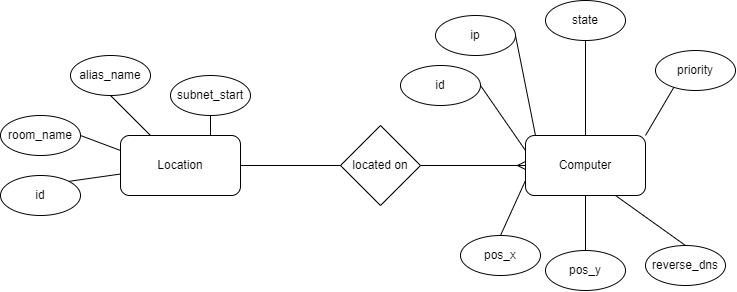
\includegraphics[width=0.75\textwidth]{images/db-loca-comp.png}
                        \caption{Entitas \textit{Location} dan entitas \textit{Computer}}
                        \label{fig:entiti-location-computer}
                    \end{figure}
                    
                    
            		Penambahan sistem manajemen ruang ini mengharuskan adanya perubahan pada bentuk entitas \textit{Location} dan entitas \textit{Computer} pada basis data. Terdapat penambahan 2 buah atribut pada entitas \textit{Computer}, yaitu \textit{state} dan \textit{priority}. Atribut \textit{state} digunakan untuk menandai status komputer di sebuah ruangan. Status sendiri terdiri dari nilai 0 atau 1. Nilai 0 berarti komputer tidak ditandai rusak oleh Tim Admin, sedangkan nilai 1 komputer ditandai sebagai komputer yang sedang rusak oleh Tim Admin. 
            		
            		Atribut \textit{priority} nantinya akan digunakan untuk melakukan pemilihan posisi ujian secara otomatis. Atribut ini digunakan untuk menyimpan skala prioritas sebuah komputer dalam pemilihan posisi ujian. Komputer dengan skala prioritas lebih kecil akan didahulukan dalam pemilihan posisi ujian.
            		 Atribut lainnya yang berubah adalah pos\_x dan pos\_y yang sebelumnya disatukan sebagai atribut d\_pos yang berisi koordinat x dan y dan disimpan dalam bentuk \textit{string} JSON.
            		 
            		 Pada entitas \textit{Location} terdapat perubahan berupa penambahan atribut subnet\_start. Atribut ini ditambahkan untuk mempermudah pengisian atribut ip pada sebuah komputer di ruangan. Sebagai contoh, pada ruangan dengan subnet\_start 192.168.10.0, komputer dengan nomor 1 akan mendapatkan IP \textit{address} 192.168.10.1. Pengisian nilai atribut ip ini akan dilakukan secara otomatis melalui sistem menajemen ruang lab ketika Tim Admin menambahkan komputer.
            		 
            		 
            		\item \textbf{Pemilihan Posisi Ujian secara Otomatis}\\
            		\label{pemilihan-otomatis}
            	    Pada saat mempersiapkan ujian, Tim Admin akan melakukan pemilihan posisi ujian yang akan digunakan oleh peserta ujian. Pada OXAM v.5.0, pemilihan posisi ujian ini dilakukan secara manual satu per satu. Menurut usulan yang diberikan, hal ini sebenarnya dapat diotomatisasi. Selain mempercepat proses persiapan ujian, juga dapat mencegah adanya \textit{human error} yang terjadi pada saat pemilihan posisi ujian. 
            	    
                     \begin{figure}[H]
                        \centering
                        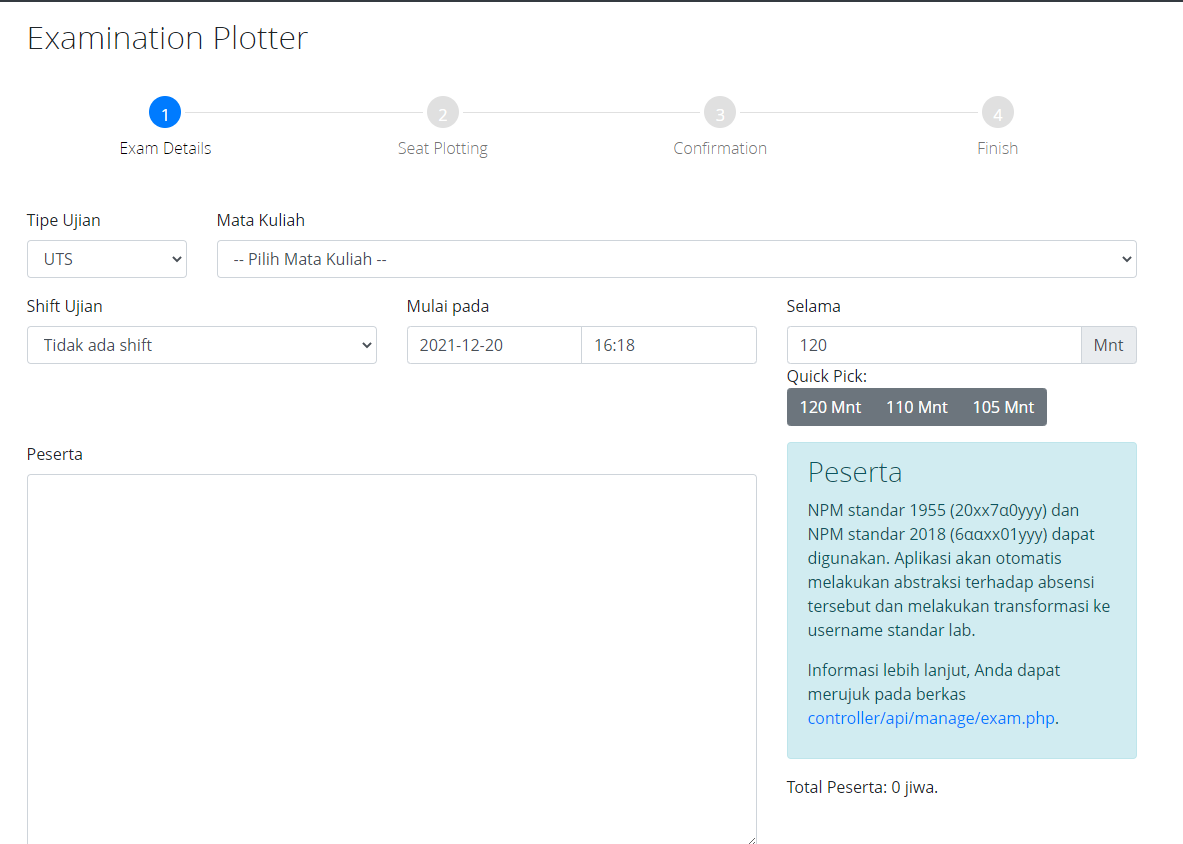
\includegraphics[width=0.75\textwidth]{images/create-exam-1.PNG}
                        \caption{Langkah pertama dalam pembuatan ujian di Lab}
                        \label{fig:create-exam-1}
                    \end{figure}
                    
            	    
            	    Setelah Tim Admin menyelesaikan langkah pertama dengan mengisi \textit{input} seperti yang terlihat pada gambar \ref{fig:create-exam-1}, Tim Admin akan diarahkan ke halaman \textit{seat plotting} yang digunakan untuk memilih posisi komputer mana saja yang dapat ditempati oleh peserta ujian. Ketika berpindah ke langkah kedua, sistem akan melakukan \textit{ping} ke komputer yang ada di lab yang terpilih secara \textit{default}, kemudian melakukan pemilihan posisi berdasarkan prioritas komputer di lab tersebut.
            	    
            	    Pemilihan juga memperhatikan \textit{status} dari komputer, jika ditandai sebagai komputer rusak oleh Admin tidak akan diikutsertakan dalam pemilihan. Selain komputer dengan status ditandai rusak, pemilihan juga akan dilewati untuk komputer yang sudah terisi peserta dengan waktu ujian yang bersinggungan dengan ujian yang sedang dibuat. Pemilihan secara otomatis ini tidak bersifat absolut, dengan artian masih dapat diubah lagi oleh Tim Admin setelah pemilihan secara otomatis selesai dilakukan. 
            	   
            	    Sama seperti sistem manajemen ruang, fitur pemilihan posisi secara otomatis ini dikhususkan untuk digunakan oleh Tim Admin. Terdapat beberapa hal yang harus dapat dilakukan oleh Tim Admin, yaitu:
            	    \begin{itemize}
            	        \item Sistem dapat melakukan \textit{auto-select} berdasarkan konfigurasi status komputer di lab oleh Tim Admin, prioritas komputer, dan memperhatikan ketersediaan komputer terkait dengan ujian lain yang sedang berlangsung
            	        \item Ketika Tim Admin melakukan pemilihan pada tab Lab, akan dilakukan \textit{auto-select} posisi berdasarkan jumlah komputer yang tersedia dan juga jumlah peserta yang ada
            	        \item Status komputer (\textit{available}, \textit{marked unavailable}, \textit{not connected}, \textit{occupied}) 
            	        \item Tim Admin dapat melakukan perubahan pada pemilihan posisi komputer yang dihasilkan oleh sistem
            	    \end{itemize}
	                
	                \vspace{0.3cm}
	    
            		\item \textbf{Sinkronisasi Status Komputer di Ruang Lab dan OXAM}\\
            		\label{sinkronisasi-status}
            	    Sinkronisasi status komputer dilakukan oleh Tim Admin dengan menandai pada sistem status komputer yang bersangkutan sesuai dengan keadaan \textit{real time}. Komputer yang sudah ditandai tidak tersedia, nantinya tidak akan diikutsertakan dalam pemilihan posisi ujian secara otomatis. Tim Admin juga dapat melakukan perubahan kembali untuk komputer yang ditandai tidak tersedia pada sistem. Sehingga dapat diikursertakan kembali dalam mekanisme pemilihan posisi ujian secara otomatis. 
            	    
            	    \vspace{0.3cm}
            	    
            	    \item \textbf{Pemindahan Posisi Ujian Peserta (Migrator)}\\
            	    \label{migrator}
            	    Fitur pemindahan posisi peserta saat ini masih dilakukan dengan cara melakukan input secara manual posisi mahasiswa yang akan dipindahkan dan juga posisi tujuan. Fitur \textit{migrator} ini dapat diubah disesuaikan untuk menggunakan mekanisme yang sama seperti pada saat melakukan pemilihan posisi ujian. Nantinya proses pemindahan posisi pada sat ujian berlangsung tidak dilakukan dengan mengetikkan NPM peserta, tapi dapat dilakukan secara interaktif. Pemindahan dapat dilakukan baik dengan cara \textit{drag} \& \textit{drop} untuk pemindahan posisi di lab yang sama, atau dengan cara klik posisi asal dan tujuan di 2 lab yang berbeda.
            	    
            	    \vspace{0.3cm}
            	    
            	    \item \textbf{Mode Ujian Berbasis Token}\\
            	    \label{mode-ujian-basis-token}
            		Seperti yang juga sudah dibahas di bagian \ref{sec:deskripsi}, ujian menggunakan OXAM saat ini hanya dapat dilakukan di ruangan lab. Hal ini dikarenakan otentikasi pada \textit{endpoint} \url{https://oxam.labftis.net/exam} hanya akan menampilkan informasi ujian apabila diakses melalui komputer yang berada di lab (IP komputer yang mengirimkan \textit{request} tercatat di \textit{database}).
            		
            		Mode ujian dengan otentikasi berbasis token ditambahkan untuk memungkinkan ujian dilakukan di luar ruang lab. Dengan demikian, waktu ujian menjadi lebih fleksibel. Ujian yang sifatnya dilakukan secara \textit{shift} dapat dilakukan bersamaan. Selain itu, dengan adanya mode ini, fungsi OXAM tidak lagi terbatas hanya untuk mengatur ujian UAS maupun UTS, namun juga dapat digunakan untuk mengatur \textit{quiz}.
            		
            		Pada mode ujian dengan otentikasi berbasis token terdapat 3 aktor yang terlibat, yaitu tim admin, dosen, dan juga peserta ujian. Pada mode ini masing-masing aktor memiliki kebutuhan tersendiri, diataranya:
            		\begin{itemize}
            		    \item Tim Admin
            		    \begin{itemize}
            		        \item Tim Admin dapat membuat ujian baru tanpa melakukan pemilihan posisi ujian
            		        \item Tim Admin dapat menyertakan file yang akan digunakan untuk ujian yang diberikan oleh Dosen yang mengampu Mata Kuliah yang akan diujikan
            		    \end{itemize}
            		    
            		    \item Dosen
            		    \begin{itemize}
            		        \item Dosen dapat melakukan login dari luar untuk membuat ujian baru
            		        \item Dosen dapat membuat ujian baru tanpa melakukan pemilihan posisi ujian
            		        \item Dosen dapat menyertakan file yang akan digunakan untuk ujian
            		        \item Fitur-fitur dari sistem Oxam lama seperti pengiriman notifikasi dan \textit{timer screen} tetap berjalan
            		    \end{itemize}
            		    \item Peserta
            		    \begin{itemize}
            		        \item Peserta ujian dapat melakukan login dari luar lab untuk melakukan ujian
            		        \item Peserta ujian dapat melakukan pengunduhan file dari ujian yang akan/sedang berlangsung dari luar lab
            		        \item Peserta ujian dapat melakukan pengumpulan jawaban dari luar lab tanpa kendala
            		        \item Fitur seperti notifikasi dan timer yang terintegrasi di sistem yang lama tetap berjalan dan berfungsi pada mode berbasis token untuk peserta
            		    \end{itemize}
            		\end{itemize}
            		
            		  \textit{Login} untuk peserta ujian dan juga dosen akan dilakukan dengan mencocokan data identitas seperti \textit{username} dan \textit{password} ke\textit{Active Directory} (AD) dengan menggunakan protokol \textit{Lightweight Directory Access Protocol} (LDAP). Jika data \textit{login}  yang disertakan sesuai dengan yang ada pada AD, maka user akan diberikan token untuk melakukan akses terkait dengan ujian.
		     \end{itemize}
		\end{itemize}
	
		\item \textbf{Merancang dan mengimplementasi perangkat lunak.}\\
		{\bf Status :} Ada sejak rencana kerja skripsi.\\
		{\bf Hasil :}
		
		\begin{itemize}
		    \item \textbf{Rancangan \textit{User Interface} (UI)}
		    \label{design-ui}
		    
		    Rancangan \textit{interface} juga turut dibuat pada tahap ini untuk mempermudah identifikasi langkah-langkah yang diperlukan masing-masing proses pada fitur yang akan dibuat.Berikut merupakan rancangan \textit{interface} yang dibuat untuk masing-masing fitur:
		    
		    \begin{itemize}
		        \item \textbf{Sistem Manajemen Ruang dan Komputer}\\
		        \setlength\parindent{24pt}
		        Menu utama baru, yaitu \textit{Location} ditambahkan pada \textit{navigation bar}  untuk memudahkan akses menuju halaman utama yang digunakan untuk melakukan manajemen ruang dan komputer. Sebelumnya, baik \textit{location} maupun \textit{computer} merupakan anak dari menu \textit{Exam params}. Beberapa alasan menu ini ditambahkan sejajar dengan menu utama adalah (1) Implementasi fitur manajemen ruang menggunakan \textit{endpoint} sebelumnya memisahkan \textit{location} dari \textit{computer}. Pada desain yang baru, ketika mengakses mengenai detail sebuah ruangan lab, maka akan ditampilkan denah dari komputer yang ada pada lab tersebut. Jika menggunakan desain \textit{endpoint} yang lama (masuk menjadi anak dari \textit{Exam params}) akan lebih sulit diaplikasikan; (2) Dengan memindahkan kedua menu tersebut ke satu menu utama, yaitu \textit{Location} perubahan \textit{endpoint} yang digunakan untuk fitur tersebut lebih bebas untuk diemplementasikan mengikuti pola \textit{endpoint} yang digunakan oleh menu \textit{Ujian}.
		        
                 \begin{figure}[H]
                    \centering
                    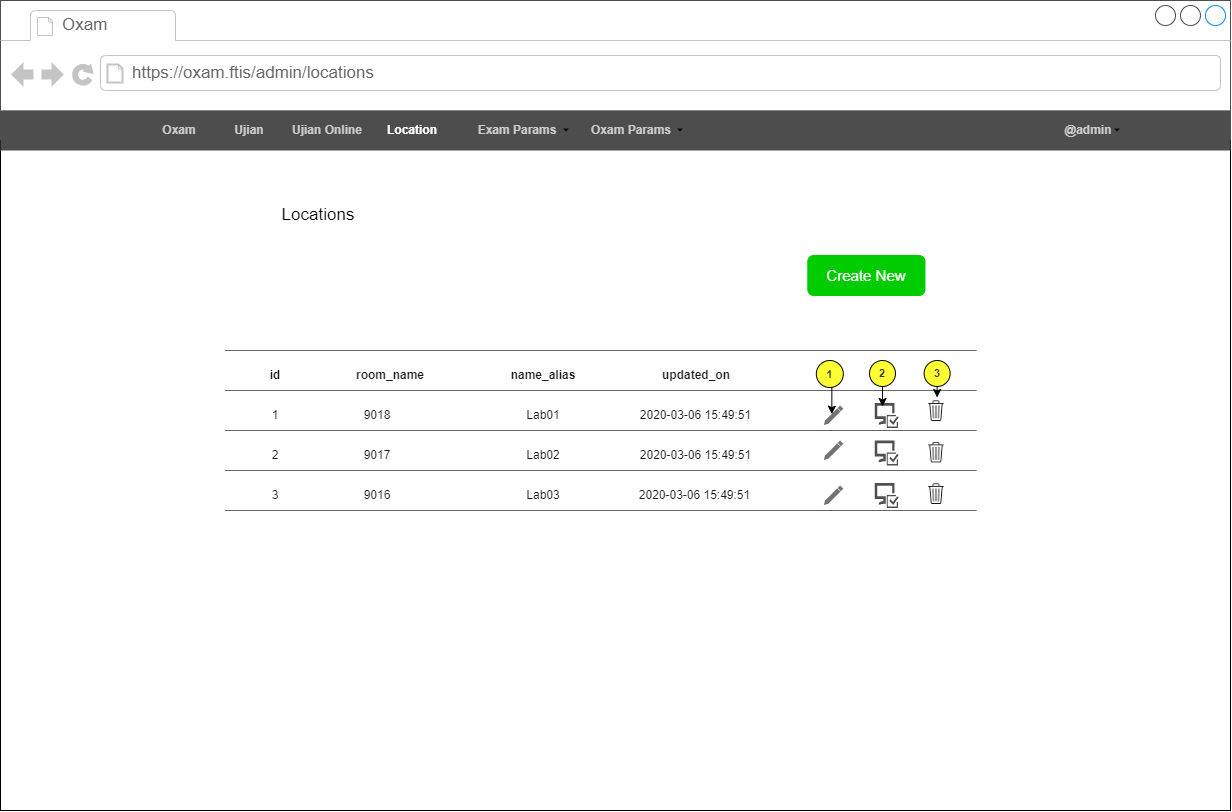
\includegraphics[width=0.8\textwidth]{images/ui designs/room-management/locations.png}
                    \caption{Halaman utama dari menu \textit{Location}.}
                    \label{fig:room-mgmt-locations}
                \end{figure}
                
                Gambar \ref{fig:room-mgmt-locations} merupakan tampilan utama yang ada pada menu utama \textit{Location}. Tampilan secara umum sama seperti tampilan yang digunakan \textit{location} sebelumnya ketika masih menjadi submenu dari \textit{Exam params}.  Terdapat tombol \textit{Create New} yang digunakan untuk menambahkan ruangan lab baru. 
                
                 \begin{figure}[H]
                    \centering
                    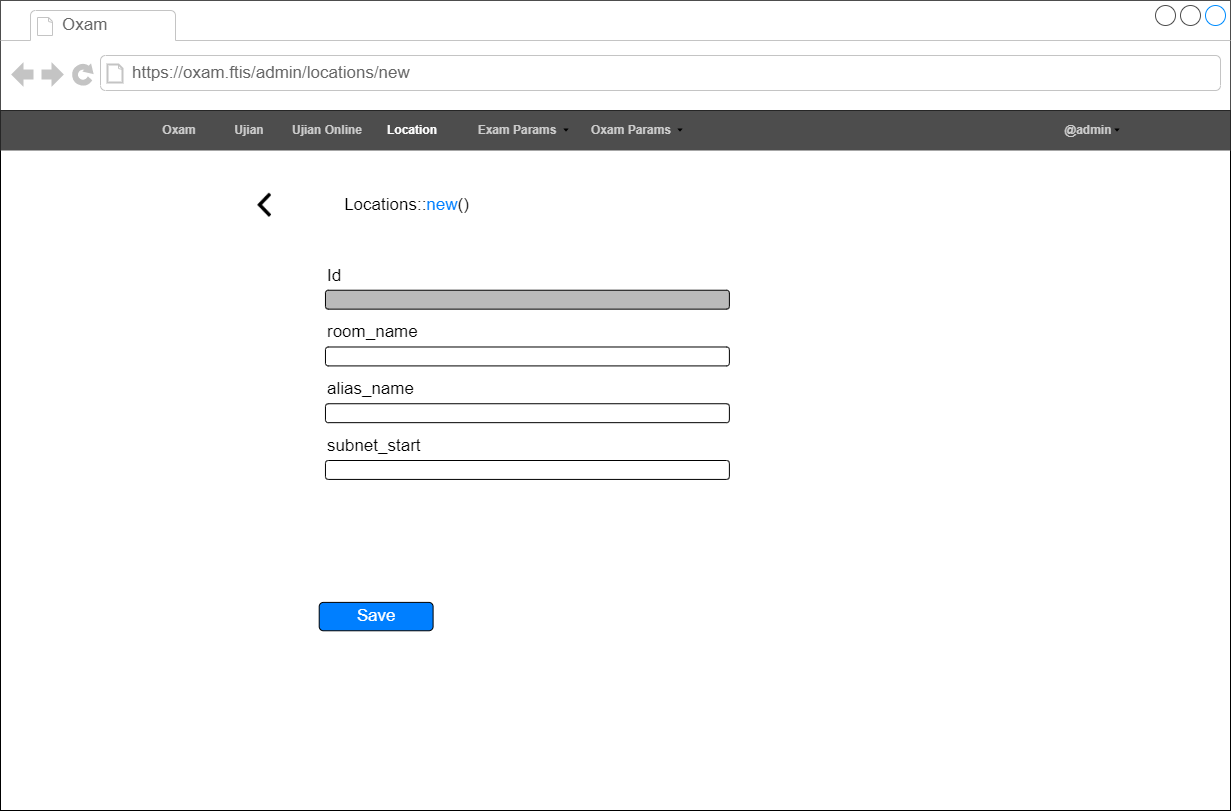
\includegraphics[width=0.8\textwidth]{images/ui designs/room-management/new-locations.png}
                    \caption{Halaman tambah ruangan baru.}
                    \label{fig:room-mgmt-new-locations}
                \end{figure}
                
                Terdapat beberapa \textit{form} masukan yang dapat diisi, yaitu \textit{room\_name}, \textit{alias\_name}, dan \textit{subnet\_start}. Nilai dari id nantinya diisi secara otomatis ketika dimasukan ke basis data, sehingga sengaja dibuat \textit{disabled}. Masukan \textit{room\_name} merupakan nomor ruangan dari sebuah ruang lab (contohnya 9017 atau 9018). Masukan \textit{alias\_name} adalah nama alias dari ruangan lab yang biasa dipakai oleh para Tim Admin (contohnya, Lab01 atau Lab02). Perbedaan yang ada pada halaman ini dibandingkan dengan halaman \textit{new location} sebelumnya adalah penambahan masukan untuk \textit{subnet\_start}. Nilai dari \textit{subnet\_start} akan digunakan untuk mengisi data IP \textit{Address} dari sebuah komputer secara otomatis, sehingga tidak perlu dituliskan secara manual ketika ditambahkan.
                
                %  \begin{figure}[H]
                %     \centering
                %     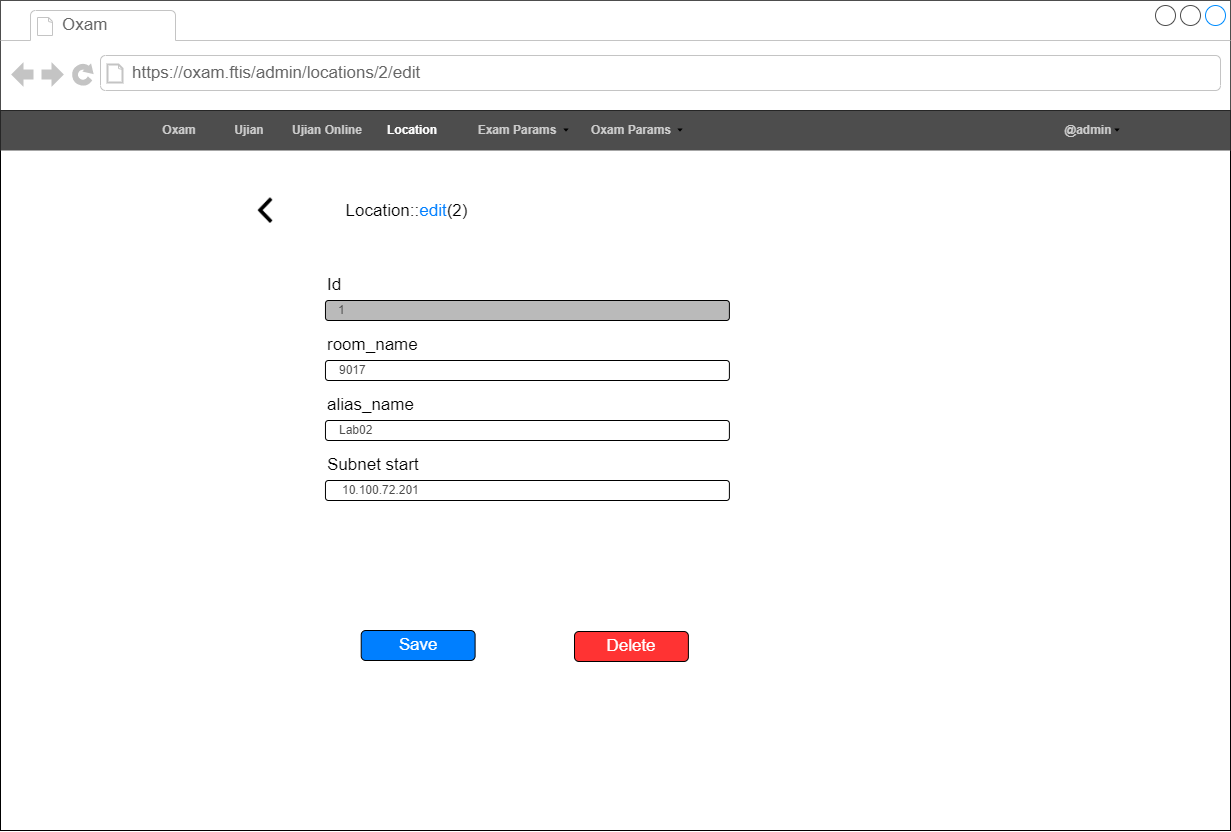
\includegraphics[width=1\textwidth]{images/ui designs/room-management/edit-locations.png}
                %     \caption{Halaman \textit{edit} untuk ruang lab 9017 atau Lab02.}
                %     \label{fig:room-mgmt-edit-location}
                % \end{figure}
                
                % Tombol dengan label 1 pada Gambar \ref{fig:room-mgmt-locations}, jika ditekan akan mengarahkan pengguna ke halaman \textit{edit} untuk ruang lab yang dipilih. Gambar \ref{fig:room-mgmt-edit-location} merupakan tampilan ketika \textit{edit} dilakukan pada sebuah ruang lab. 
                
                 \begin{figure}[ht]
                    \centering
                    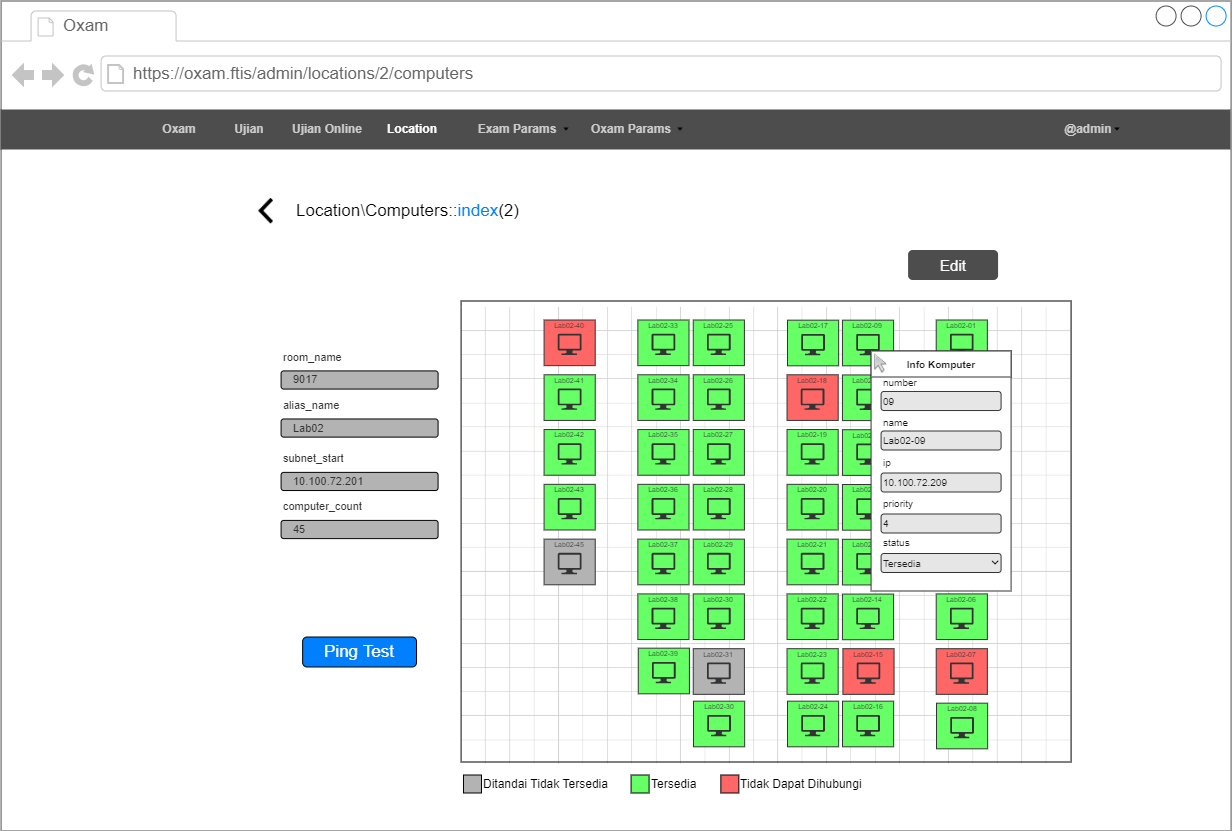
\includegraphics[width=0.9\textwidth]{images/ui designs/room-management/location-id2.png}
                    \caption{Halaman detail komputer dari ruang lab 9017 atau Lab02.}
                    \label{fig:room-mgmt-detail-computers}
                \end{figure}
                
                 Tombol dengan label 1 pada Gambar \ref{fig:room-mgmt-locations}, jika ditekan akan mengarahkan pengguna ke halaman \textit{edit} untuk ruang lab yang dipilih. Perbedaan dari tampilan sebelumnya terletak pada tombol dengan \textit{icon} komputer yang ditandai menggunakan label 2 pada Gambar \ref{fig:room-mgmt-locations}. Ketika tombol tersebut ditekan, akan mengarahkan pengguna menuju halaman detail dari ruangan lab yang dipilih serta menunjukan denah dari komputer yang ada pada ruangan lab. Tampilan tersebut dapat dilihat pada Gambar \ref{fig:room-mgmt-detail-computers}.
                
                Pada halaman detail ruang lab terdapat tombol \textit{Ping Test} yang dapat digunakan untuk melakukan \textit{test ping} ke komputer yang ada di ruang lab tersebut. Terdapat beberapa indikator yang digunakan untuk menandakan status komputer pada sebuah ruangan lab. Komputer yang ditandai dengan \textit{background} merah menandakan bahwa komputer tersebut tidak merespon ketika dilakukan \textit{ping}. Komputer dengan \textit{background} hijau menandakan bahwa komputer tersebut merespon ketika dilakukan \textit{ping}. Sedangkan komputer dengan \textit{background} berwarna abu-abu menandakan bahwa komputer tersebut ditandai oleh Tim Admin sebagai komputer yang tidak dapat digunakan (komputer rusak atau komputer secara fisik tidak ada).
                
                  \begin{figure}[H]
                    \centering
                    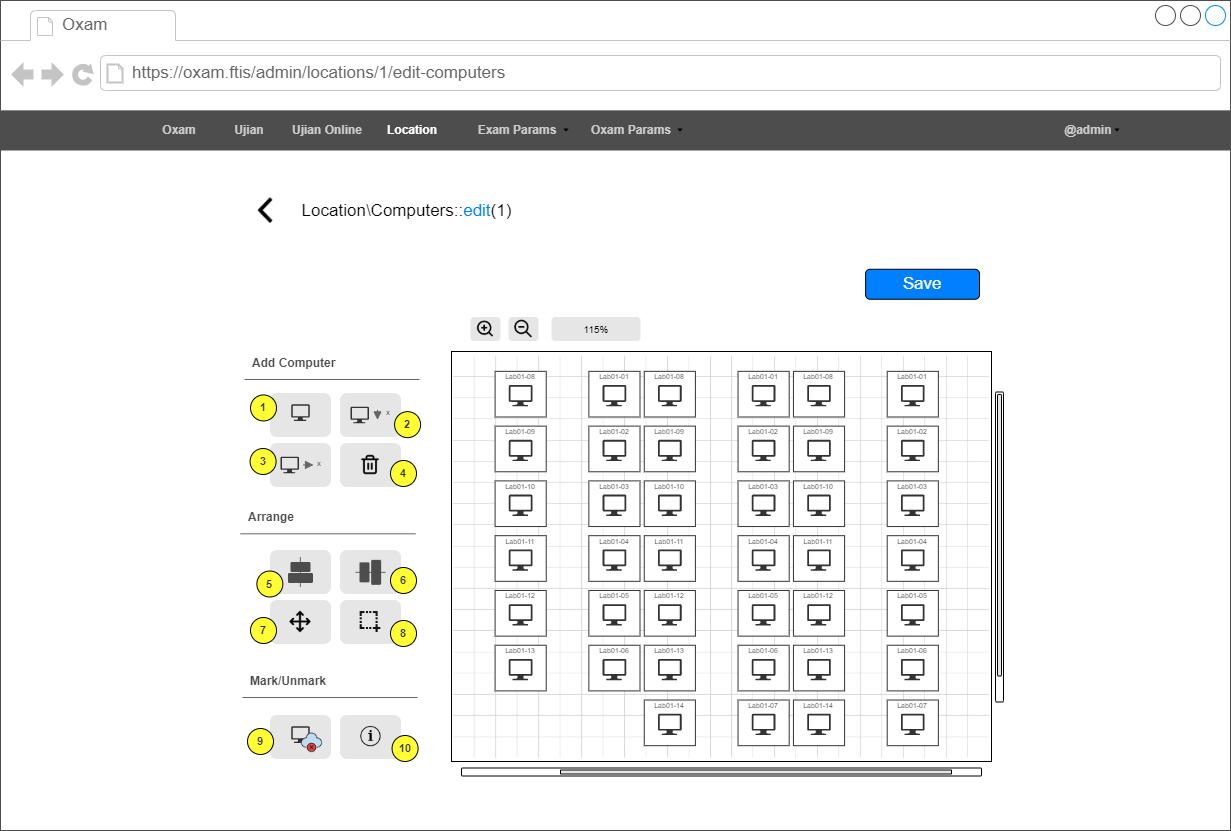
\includegraphics[width=0.9\textwidth]{images/ui designs/room-management/edit-computers.png}
                    \caption{Halaman edit ruangan lab secara interaktif.}
                    \label{fig:room-mgmt-edit-computers}
                \end{figure}
                
                Selain tombol \textit{ping}, terdapat tombol \textit{Edit} yang jika ditekan akan mengarahkan menuju halaman \textit{edit} \textit{layout} komputer di ruangan lab yang dipilih. Tampilan dari halaman untuk melakukan \textit{edit} layout dari ruangan lab dapat dilihat pada Gambar \ref{fig:room-mgmt-edit-computers}. Terdapat beberapa tombol yang disediakan untuk memudahkan perubahan layout pada ruangan lab.
                
                
                  \begin{figure}[H]
                    \centering
                    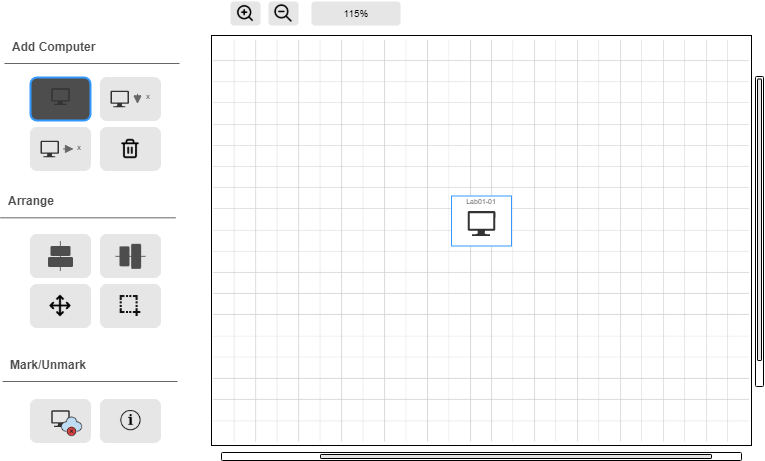
\includegraphics[width=0.75\textwidth]{images/ui designs/room-management/add-single-1.png}
                    \caption{Komputer yang ditambahkan secara otomatis ke tengah-tengah kanvas ketika tombol tambah komputer ditekan.}
                    \label{fig:room-mgmt-edit-computers-add-single}
                \end{figure}
                
                
                Tombol dengan label 1 pada Gambar \ref{fig:room-mgmt-edit-computers} digunakan untuk menambahkan komputer ke dalam \textit{layout} ruangan. Jika tombol ini ditekan, maka akan menambahkan secara otomatis sebuah komputer ke dalam denah seperti yang terlihat pada Gambar \ref{fig:room-mgmt-edit-computers-add-single}. Ketika komputer ditambahkan, data-data terkait dengan komputer tersebut seperti nomor komputer, \textit{dns\_reverse}/nama komputer, IP \textit{Address}, dan koordinat dari komputer pada denah akan dihasilkan secara otomatis. Selain data-data tadi, status awal komputer akan dibuat menjadi \textit{available}/tersedia dan diberikan nilai prioritas satu (1).
                
                  \begin{figure}[H]
                    \centering
                    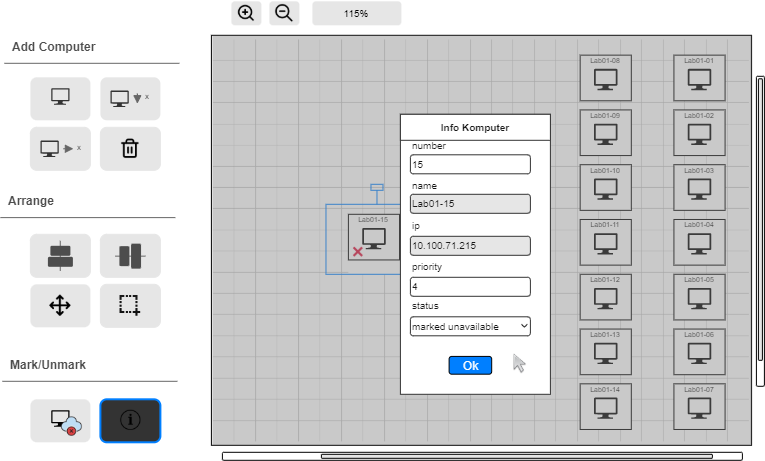
\includegraphics[width=0.75\textwidth]{images/ui designs/room-management/info.png}
                    \caption{Tombol \textit{info} untuk melihat detail dari sebuah komputer pada denah.}
                    \label{fig:room-mgmt-edit-computers-info}
                \end{figure}
                
                Info dari sebuah komputer yang sudah ditambahkan ke denah dapat dilihat dengan cara menekan tombol info (tombol dengan label nomor 10 pada Gambar \ref{fig:room-mgmt-edit-computers}), kemudian memilih komputer yang akan dilihat infonya. Info dari sebuah komputer akan ditampilkan seperti yang terlihat pada Gambar \ref{fig:room-mgmt-edit-computers-info}. Pada bagian ini, perubahan dapat dilakukan pada detail data komputer dan akan disimpan ketika tombol ``Ok'' ditekan.
                
                
                  \begin{figure}[H]
                    \centering
                    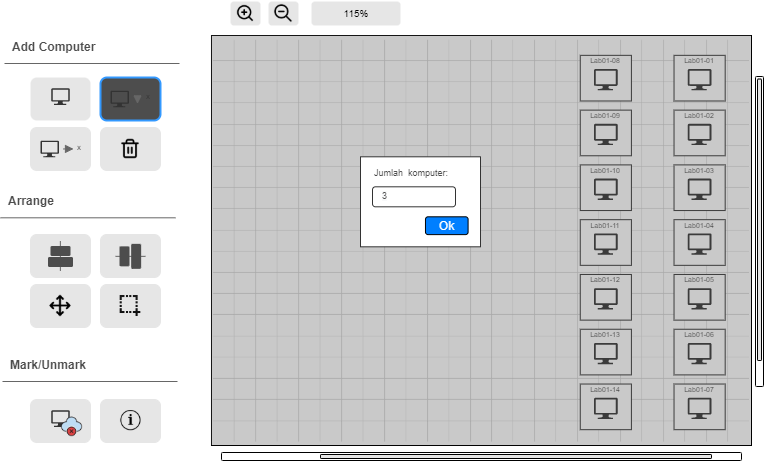
\includegraphics[width=0.75\textwidth]{images/ui designs/room-management/insert-hor.png}
                    \caption{Ketika tombol untuk menambahkan komputer dalam jumlah banyak ditekan, akan muncul \textit{prompt} untuk memasukan jumlah komputer yang akan ditambahkan.}
                    \label{fig:room-mgmt-edit-computers-add-ver-bef}
                \end{figure}
                
                  \begin{figure}[H]
                    \centering
                    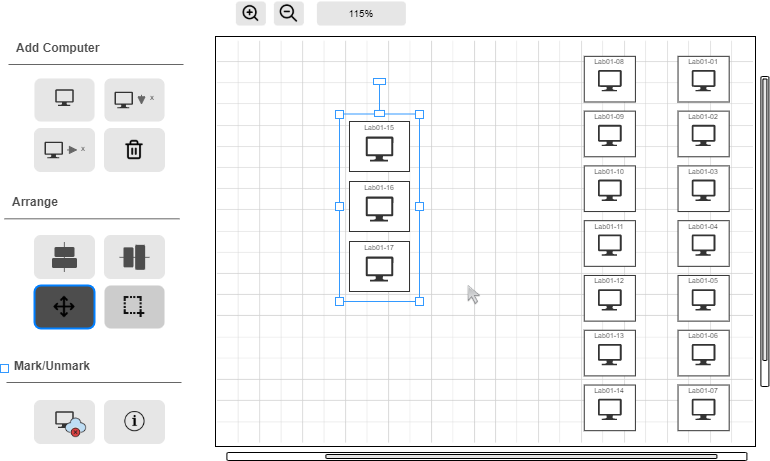
\includegraphics[width=0.75\textwidth]{images/ui designs/room-management/insert-hor-2.png}
                    \caption{Tiga buah komputer yang ditambahkan dengan pilihan orientasi yang diatur secara vertikal.}
                    \label{fig:room-mgmt-edit-computers-add-ver-aft}
                \end{figure}
                
                Selain penambahan komputer satu per satu, terdapat pula tombol untuk menambahkan komputer dalam jumlah banyak. Pada Gambar \ref{fig:room-mgmt-edit-computers}, tombol dengan label nomor 2 digunakan untuk menambahkan komputer dalam jumlah banyak dengan susunan yang diatur secara vertikal. Ketika tombol ini ditekan maka akan memunculkan \textit{prompt} untuk memasukkan jumlah komputer yang akan ditambahkan seperti yang terlihat pada Gambar \ref{fig:room-mgmt-edit-computers-add-ver-bef}. Setelah jumlah komputer yang akan ditambahkan diisi dan tombol ``Ok'' ditekan, maka komputer akan ditambahkan seperti yang terlihat pada Gambar \ref{fig:room-mgmt-edit-computers-add-ver-aft}. 
                
                Terdapat pula tombol untuk menambahkan komputer dalam jumlah banyak dengan susunan yang diatur secara horizontal (tombol dengan label nomor 3 pada Gambar \ref{fig:room-mgmt-edit-computers}). Tombol dengan \textit{icon trash can} atau tombol dengan label nomor 4 pada Gambar \ref{fig:room-mgmt-edit-computers} digunakan untuk menghapus komputer dari denah.
                
                
                \begin{figure}[H]
                \centering
                 \subfloat[]{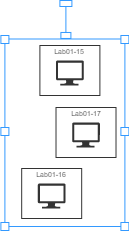
\includegraphics[width=0.2\textwidth]{images/ui designs/room-management/unaligned-ver.png}\label{fig:room-mgmt-unaligned-ver}}
                 \hfill
                 \subfloat[]{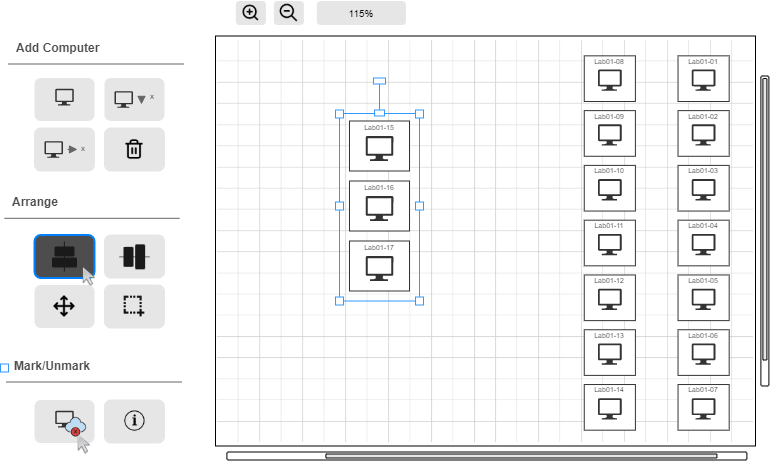
\includegraphics[width=0.65\textwidth]{images/ui designs/room-management/align-ver.png}\label{fig:room-mgmt-aligned-ver}}
                 \caption{Tombol \textit{align vertically} yang digunakan untuk merapihkan komputer yang dipilih dari keadaan pada Gambar \ref{fig:room-mgmt-unaligned-ver} menjadi lebih rapih seperti yang terlihat pada Gambar \ref{fig:room-mgmt-aligned-ver}.}
                 \label{fig:room-mgmt-aligning-ver}
                \end{figure}
                
                Selain tombol untuk menambahkan dan menghapus komputer, terdapat tombol-tombol yang dapat digunakan untuk mengatur posisi komputer secara berkelompok. Tombol dengan label nomor 5 dan 6 pada Gambar \ref{fig:room-mgmt-edit-computers} memiliki fungsi secara berurut mengatur posisi komputer agar sejajar vertikal dan sejajar horizontal. Gambar \ref{fig:room-mgmt-aligning-ver} merupakan contoh pengaturan posisi komputer-komputer yang dipilih kemudian disejajarkan secara vertikal menggunakan tombol \textit{align vertically}.
                
                Kedua tombol lainnya yang digunakan untuk mengatur posisi adalah tombol  \textit{move} (tombol dengan label nomor 7 pada Gambar \ref{fig:room-mgmt-edit-computers}) dan tombol \textit{select} (tombol dengan label nomor 8 pada Gambar \ref{fig:room-mgmt-edit-computers}).Fungsi tombol \textit{select} digunakan untuk memilih sebuah komputer atau dapat pula memilih kumpulan komputer. Tombol \textit{move} kemudian dapat digunakan untuk memindahkan komputer yang telah terpilih ke posisi baru. 
                
                
                  \begin{figure}[H]
                    \centering
                    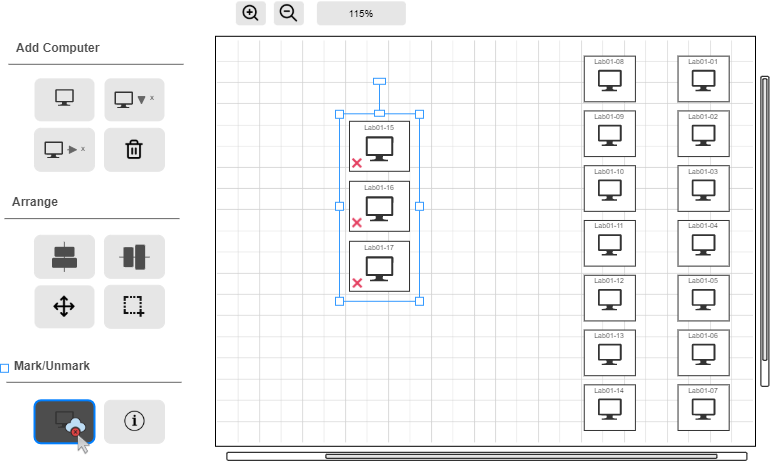
\includegraphics[width=0.75\textwidth]{images/ui designs/room-management/mark-unavailable.png}
                    \caption{Tiga buah komputer yang terpilih ditandai sebagai komputer yang tidak dapat digunakan untuk ujian di ruangan lab.}
                    \label{fig:room-mgmt-edit-computers-mark-unavail}
                \end{figure}
                
                Tombol yang terakhir adalah tombol \textit{mark} yang dapat digunakan untuk memberi tanda kepada komputer sebagai komputer yang tidak dapat digunakan untuk ujian. Komputer-komputer yang terpilih berubah status menjadi \textit{not available} ketika tombol ini ditekan seperti yang terlihat pada Gambar \ref{fig:room-mgmt-edit-computers-mark-unavail}. Jika sebelumnya komputer sudah ditandai sebagai komputer yang tidak dapat digunakan (not available) dan tombol ini ditekan, maka tanda tersebut akan dihilangkan dan status komputer berganti menjadi dapat digunakan untuk ujian.
                \\
                
		        \item \textbf{Pemilihan Posisi Ujian secara Otomatis}\\
		        \setlength\parindent{24pt}
		        Salah satu hal yang dilakukan oleh Tim Admin ketika mempersiapkan ujian di ruang lab adalah mendaftarkan entri ujian ke OXAM. Untuk mendaftarkan sebuah ujian Tim Admin akan mengisi \textit{form} pembuatan ujian yang ada pada OXAM. Terdapat 4 tahap dalam pengisian \textit{form} pembuatan ujian pada OXAM, yaitu pengisian detail ujian (\textit{exam details}), pengalokasian tempat duduk untuk ujian (\textit{seat plotting}), konfirmasi ujian (\textit{confirmation}), dan penyelesaian (\textit{finish}). Sistem \textit{seat plotting} pada OXAM v.5.0 atau versi saat ini mengharuskan Tim Admin untuk melakukan pemilihan posisi ujian secara manual dengan memilih satu per satu komputer yang akan digunakan. Hal ini selain memakan waktu, juga rentan terhadap \textit{human error}. 
		        
		        Pada rancangan \textit{seat plotting} yang baru, akan diintegrasikan dengan pengaturan yang ada pada sistem manajemen ruang dan komputer. Pemilihan posisi kini akan dilakukan secara otomatis dan pemilihannya ditentukan berdasarkan nilai prioritas dari komputer serta status dari komputer yang sebelumnya telah diatur oleh Tim Admin sebelum pengisian entri ujian dilakukan.
		        
                \begin{figure}[H]
                    \centering
                    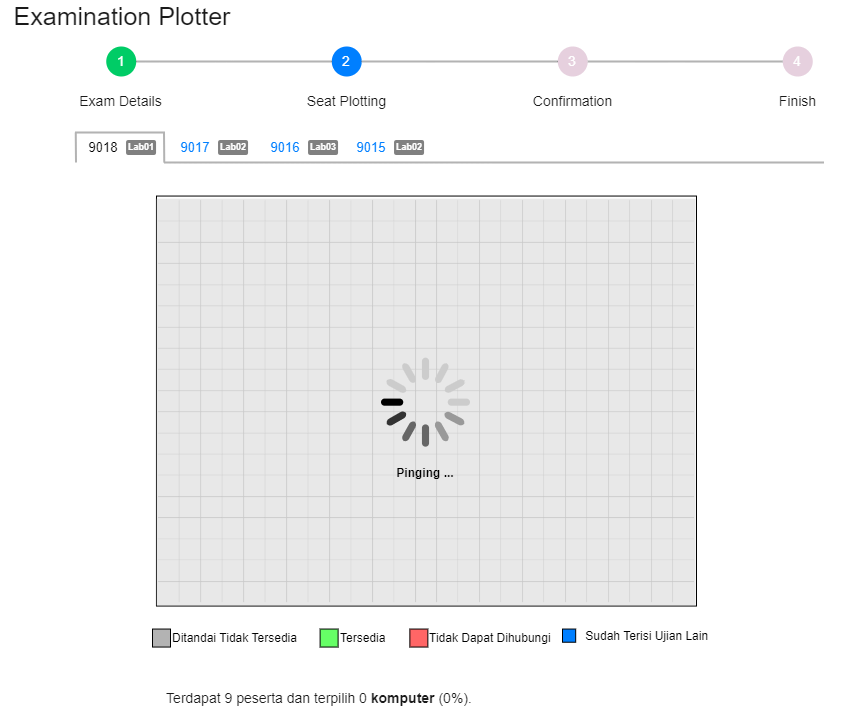
\includegraphics[width=0.75\textwidth]{images/ui designs/automation/step-2-1-ping-2.png}
                    \caption{Proses \textit{ping} komputer yang berada di ruangan 9018 pada tahap kedua pembuatan entri ujian.}
                    \label{fig:automation-ping-2}
                \end{figure}
                
		        Tahap \textit{seat plotting} akan diawali dengan proses \textit{ping} ke komputer yang berada di sebuah ruang lab. Proses \textit{ping} hanya akan dilakukan satu kali pada saat sebuah ruangan lab dipilih  agar tidak memakan waktu terlalu lama. Seperti yang terlihat pada Gambar \ref{fig:automation-ping-2}, tab untuk ruang 9018 terpilih secara \textit{default}, sehingga akan dilakukan \textit{ping} untuk komputer yang berada di ruangan ini.
		        
                \begin{figure}[H]
                    \centering
                    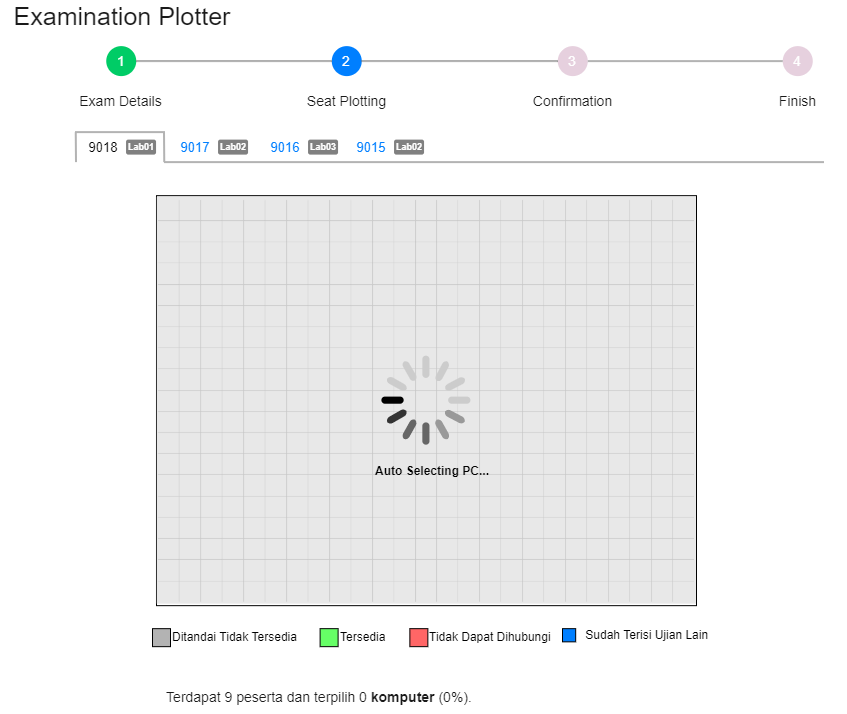
\includegraphics[width=0.77\textwidth]{images/ui designs/automation/step-2-2-autoselect-2.png}
                    \caption{Proses pemilihan posisi ujian secara otomatis berdasarkan nilai prioritas komputer dan juga status dari komputer.}
                    \label{fig:automation-autoselect-2}
                \end{figure}
		        
		        Setelah proses ping selesai dilakukan, maka akan dilakukan proses pemilihan posisi ujian secara otomatis berdasarkan nilai prioritas dari komputer serta status dari sebuah komputer. Proses ini ditandai dengan \textit{loading screen} yang terlihat pada Gambar \ref{fig:automation-autoselect-2}. Nilai prioritas sebuah komputer dimulai dari nilai satu (1) sebagai prioritas tertinggi. Komputer yang tersedia dan belum terpilih dengan nilai prioritas rendah akan selalu diutamakan dalam pemilihan posisi ujian. 
		        
		        Terdapat 4 jenis status yang juga akan digunakan sebagai parameter untuk pemilihan posisi ujian. Komputer yang nantinya ditandai dengan \textit{background} berwarna abu-abu merupakan komputer dengan status ditandai tidak tersedia (\textit{marked not available}) oleh Tim Admin, sehingga secara otomatis tidak akan diikutsertakan dalam pemilihan posisi ujian. Komputer dengan \textit{background} berwarna hijau merupakan komputer yang berhasil memberikan balasan pada proses \textit{ping} dan merupakan kandidat yang dapat digunakan untuk pemilihan posisi ujian. Komputer dengan  \textit{background} berwarna merah merupakan komputer yang tidak memberikan balasan ketika proses \textit{ping} dilakukan, sehingga tidak akan digunakan. Sedangkan komputer dengan \textit{background} berwarna biru merupakan komputer yang sudah terisi ujian oleh peserta dari ujian lain dengan waktu dan durasi yang sama dengan ujian yang akan dibuat.
		        
                \begin{figure}[ht]
                    \centering
                    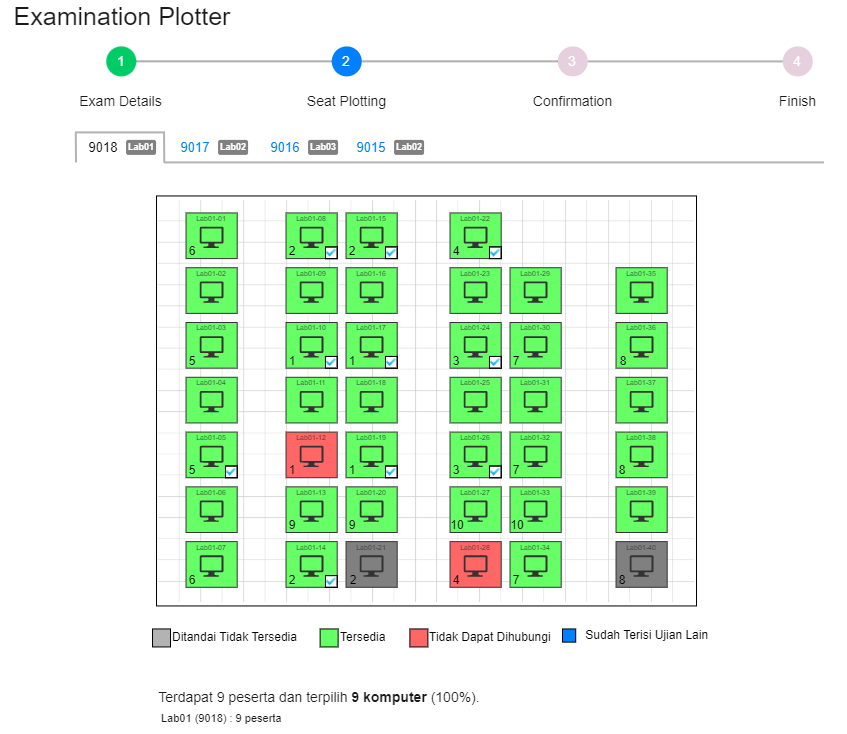
\includegraphics[width=0.8\textwidth]{images/ui designs/automation/step-2-3-selected-1.png}
                    \caption{Komputer yang terpilih untuk digunakan sebagai posisi ujian memiliki tanda \textit{checklist}.}
                    \label{fig:automation-autoselect-selected}
                \end{figure}
		        
		        Gambar \ref{fig:automation-autoselect-selected} merupakan tampilan setelah proses pemilihan posisi ujian secara otomatis selesai dilakukan. Komputer yang terpilih ditandai dengan tandan \textit{checklist}. Hasil pemilihan ini nantinya masih dapat diubah lagi oleh Tim Admin. Jika dilihat pada Gambar \ref{fig:automation-autoselect-selected} komputer yang memiliki nilai prioritas (angka di sebelah kiri bawah komputer) terletak saling terpisah 1 komputer. Pengaturan kandidat untuk pemilihan posisi ujian sengaja dibuat seperti ini untuk mengatasi adanya tindakan curang pada saat ujian. Selain itu, dengan pengaturan posisi dengan selang satu (1) dapat memudahkan Pengawas ketika mengawasi ujian.
		        
		        Komputer dengan nilai prioritas 9 dan 10 pada Gambar \ref{fig:automation-autoselect-selected} merupakan komputer yang diberikan sekat pada sisi kiri dan kanannya. Komputer yang diberikan sekat hanya akan digunakan apabila komputer dengan posisi berselang satu sudah penuh terisi. Pengaturan posisi dengan selang satu ini nantinya akan ditentukan Tim Admin melalui sistem manajemen ruang dan komputer dengan cara memberikan nilai prioritas pada komputer. Tiap lab memiliki pengaturan yang berbeda, hal ini dipengaruhi oleh jumlah komputer yang ada pada ruangan lab dan juga layout dari ruangan lab.
		        
		        Jika diperhatikan lebh lanjut pada Gambar \ref{fig:automation-autoselect-selected}, komputer nomor 12 (Lab01-12) memiliki nilai prioritas satu (prioritas tertinggi). Namun komputer ini tidak dipilih, karena tidak memberikan respon balik pada proses \textit{ping}. Begitu pula dengan komputer bernomor 21 (Lab01-21) yang tidak dipilih walaupun memiliki nilai prioritas 2 (prioritas tertinggi kedua), karena ditandai oleh Tim Admin sebagai komputer yang rusak atau komputer yang tidak tersedia secara fisik.
		        \\
		      %  \item \textbf{Sinkronisasi Status Komputer di Ruang Lab dan OXAM}
		      %  \setlength\parindent{24pt}
		        \item \textbf{Pemindahan Posisi Ujian Peserta (Migrator)}
		        \setlength\parindent{24pt}\\
		        
		        Pada saat ujian berlangsung, tidak jarang terjadi kendala seperti komputer yang mendadak bermasalah. Hal ini mengharuskan peserta ujian untuk pindah ke komputer lain agar dapat melanjutkan ujian. Pada OXAM v.5.0, terdapat \textit{migrator} yang digunakan untuk memindahkan posisi ujian peserta pada saat ujian sedang berlangsung. Pada saat akan melakukan pemindahan posisi ujian peserta, Tim Admin akan menginput nomor NPM peserta yang akan dipindahkan dan komputer tujuan pemindahan. 
		        
                \begin{figure}[H]
                    \centering
                    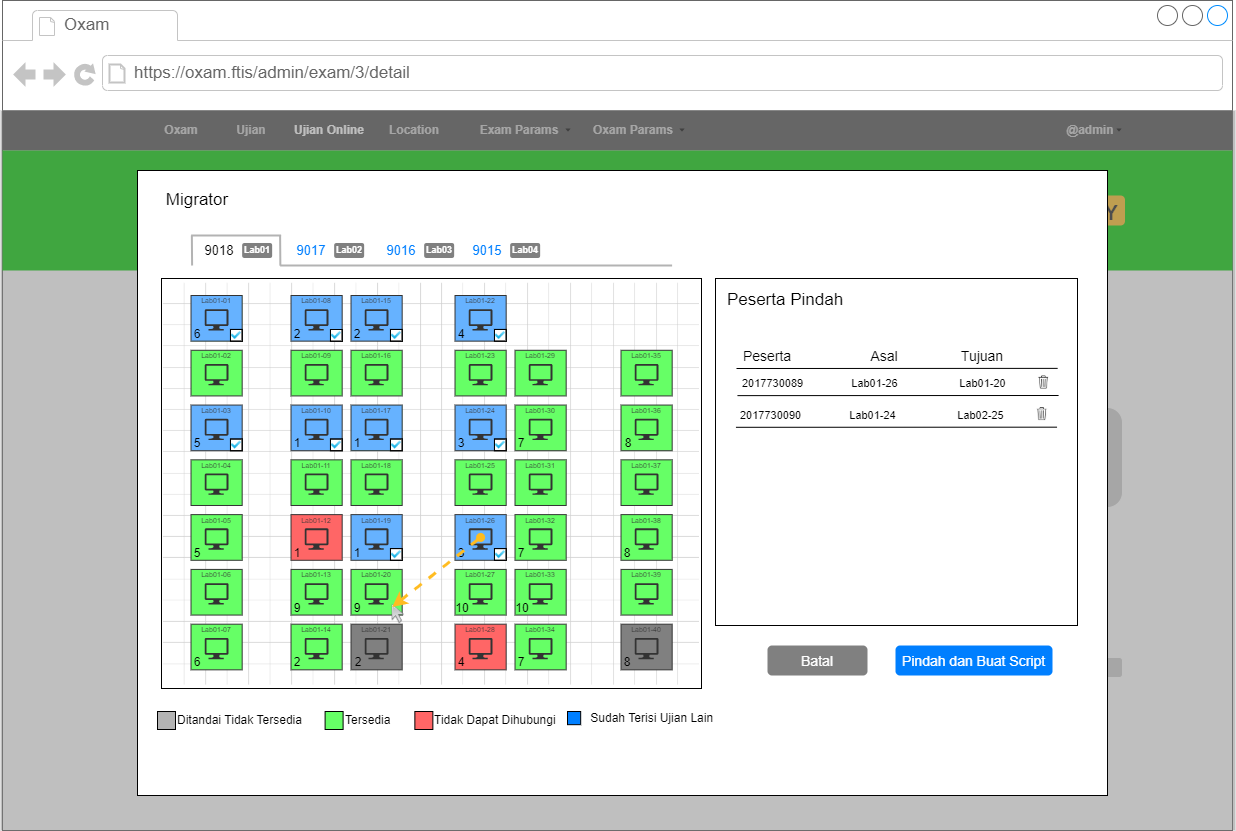
\includegraphics[width=0.9\textwidth]{images/ui designs/migrator/migrator.png}
                    \caption{\textit{Migrator} yang digunakan untuk memindahkan posisi ujian peserta pada saat ujian sedang berlangsung.}
                    \label{fig:migration-migrator}
                \end{figure}
                
                Pada fitur yang baru, pemindahan posisi ujian menggunakan migrator di ruangan yang sama dapat menggunakan \textit{drag} dari posisi asal dan \textit{drop} di posisi tujuan seperti yang terlihat pada Gambar \ref{fig:migration-migrator}. Perpindahan posisi ke ruang lab yang berbeda dapat dilakukan dengan cara klik posisi asal, kemudian klik posisi tujuan di ruangan lab lainnya. Hasil perpindahan akan tercatat di kolom \textit{list} yang ada di sebelah kanan. Setelah hasil perpindahan dikonfirmasi dan tombol ``Pindah dan Buat Script'' ditekan, maka script untuk memindahkan posisi ujian peserta akan dibuat kemudian dapat dijalankan.\\
                
		        \item \textbf{Mode Ujian dengan Otentikasi Berbasis Token}\\
		        \setlength\parindent{0pt}
		        Pada mode ujian dengan otentikasi berbasis ujian dapat dilakukan dari luar ruangan lab. Ujian dengan mode ini dapat dipersiapakan oleh Tim Admin maupun Tim Dosen dan nantinya akan diikuti oleh peserta dengan mengakses halaman exam online melalui laptop atau komputer yang dimiliki peserta.
		        \\
		        \\
		        \newpage
		        \textbf{Tampilan Antarmuka untuk Peserta}\\
		        Peserta dapat melakukan akses ujian dengan mengunjungi alamat \url{https://oxam.labfti.net/exam-online}. Ketika mengunjungi halaman ini, peserta ujian diharuskan untuk melakukan \textit{login} terlebih dahulu.
		        
                \begin{figure}[H]
                    \centering
                    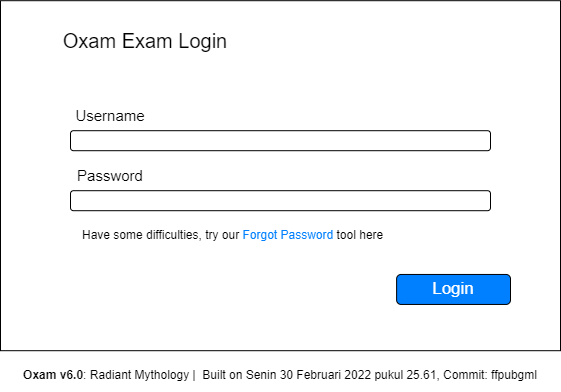
\includegraphics[width=0.65\textwidth]{images/ui designs/exam-online/login-2.png}
                    \caption{Halaman \textit{login} untuk peserta ujian.}
                    \label{fig:exam-online-login}
                \end{figure}
                
		        \setlength\parindent{24pt}
		        Setelah mengisi \textit{form login} seperti yang terlihat pada Gambar \ref{fig:exam-online-login}, data \textit{login} peserta akan dicocokan dengan data peserta yang ada pada \textit{Active Directory} (AD). Jika pasangan \textit{username} dan \textit{password} sesuai, maka peserta akan diberikan token yang digunakan untuk mengakses ujian.
		        
		        
                \begin{figure}[H]
                    \centering
                    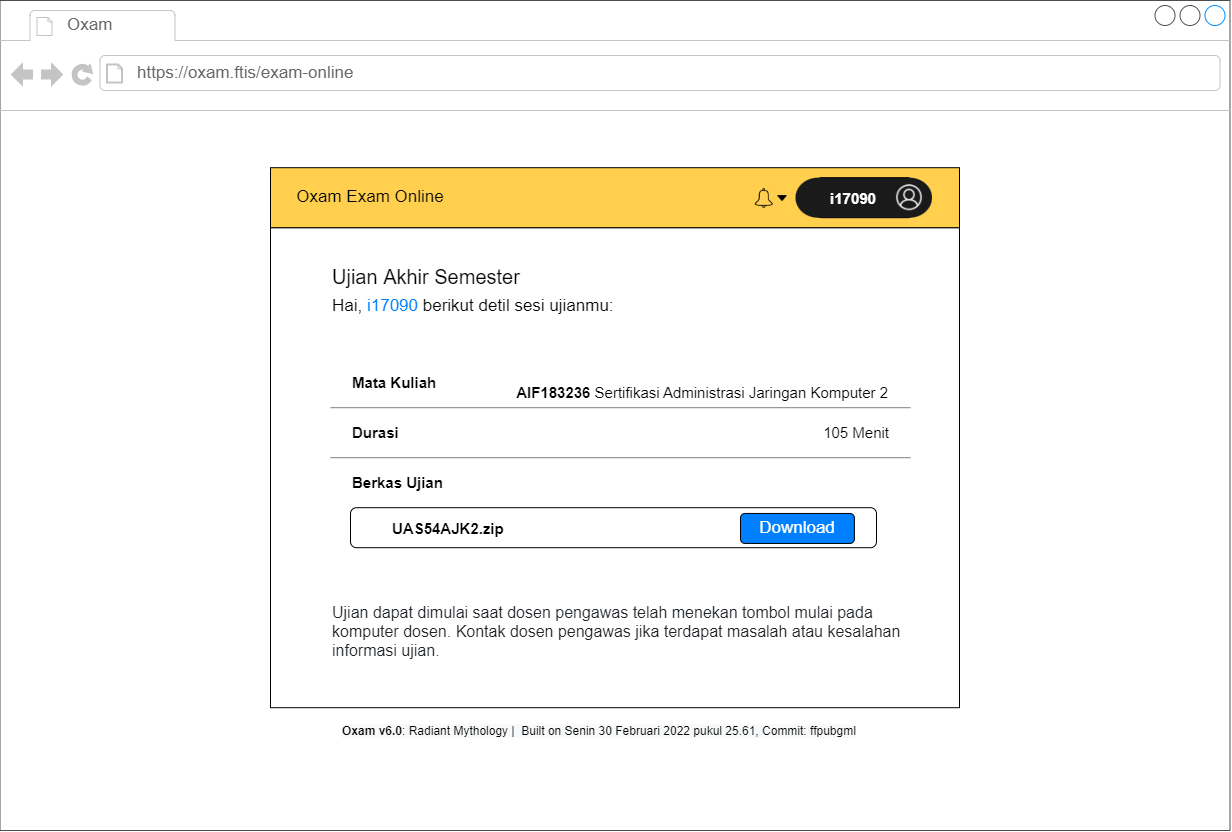
\includegraphics[width=0.9\textwidth]{images/ui designs/exam-online/exam-logged-in.png}
                    \caption{Halaman yang akan tampil setelah peserta melakukan \textit{login} pada saat ujian akan berlangsung. }
                    \label{fig:exam-online-logged-in}
                \end{figure}
		        
		        Pada ujian yang berlangsung di ruangan lab, berkas ujian didistribusikan ke komputer menggunakan \textit{script}. Berbeda dengan mode ujian dengan otentikasi berbasis token, berkas ujian akan disertakan dalam bentuk \textit{downloadable file}. Pada Gambar \ref{fig:exam-online-logged-in} dapat dilihat pada baris ``Berkas Ujian'' terdapat tombol \textit{Download} yang dapat digunakan untuk melakukan unduh berkas ujian yang disertakan oleh Tim Admin atau Dosen pada saat membuat ujian dengan mode berbasis token.
		        
		        
                \begin{figure}[ht]
                    \centering
                    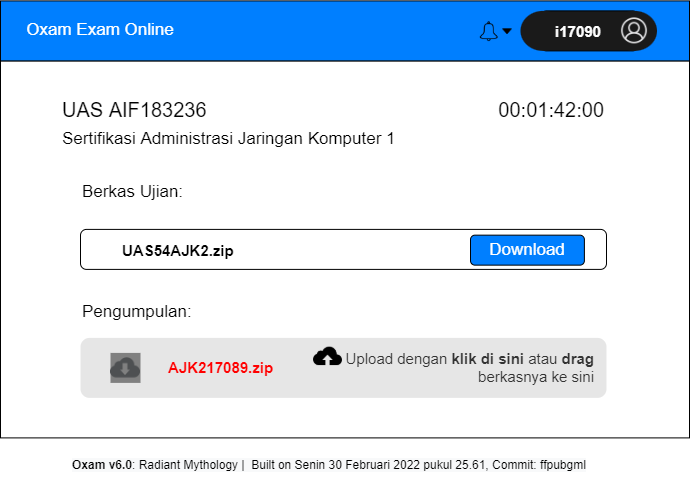
\includegraphics[width=0.6\textwidth]{images/ui designs/exam-online/exam-started-2.png}
                    \caption{Halaman yang akan tampil setelah peserta melakukan \textit{login} pada saat ujian sedang berlangsung. }
                    \label{fig:exam-online-exam-started}
                \end{figure}
		        
		        Gambar \ref{fig:exam-online-exam-started} merupakan tampilan ketika peserta berhasil melakukan \textit{login} dan ujian sudah dimulai oleh Dosen. Berkas ujian tetap disertakan, sehingga dapat diunduh kembali ketika dibutuhkan.
		        \\
		        \\
		        \textbf{Tampilan Antarmuka untuk Dosen dan Tim Admin}\\
		        Tim Admin dan juga Dosen dapat membuat entri baru untuk ujian dengan mode berbasis token. Sebelumnya dapat menambahkan entri baru, baik Tim Admin maupun Dosen harus melakukan \textit{login} terlebih dahulu melalui halaman otentikasi yang ada pada alamat \url{https://oxam.labftis.net/admin}, kemudian mengakses menu utama ``Ujian Online'' untuk mulai menambahkan entri ujian.
		        
                \begin{figure}[ht]
                    \centering
                    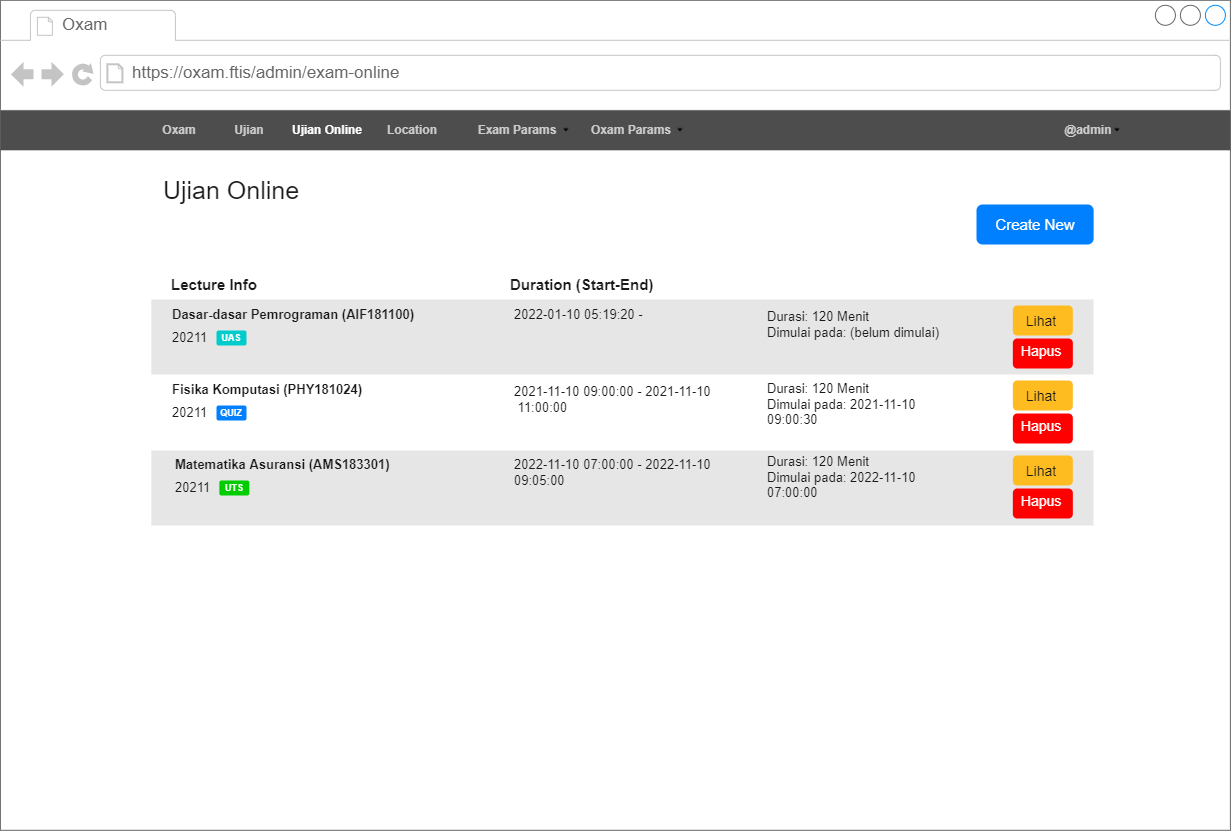
\includegraphics[width=0.8\textwidth]{images/ui designs/exam-online/manage-exam-index.png}
                    \caption{Halaman utama untuk menu utama ``Ujian Online'' . }
                    \label{fig:exam-online-manage-index}
                \end{figure}
		        
		        Gambar \ref{fig:exam-online-manage-index} merupakan tampilan untuk menu utama ``Ujian Online''. Tim Admin maupun Dosen dapat menambahkan entri baru ujian dengan menekan tombol ``\textit{Create New}''. Terdapat 3 buah label berbeda untuk menandai jenis entri ujian, yaitu label dengan warna biru muda untuk UTS, label hijau untuk UAS, dan label dengan warna biru tua untuk Quiz .
		        
		        \newpage
                \begin{figure}[H]
                    \centering
                    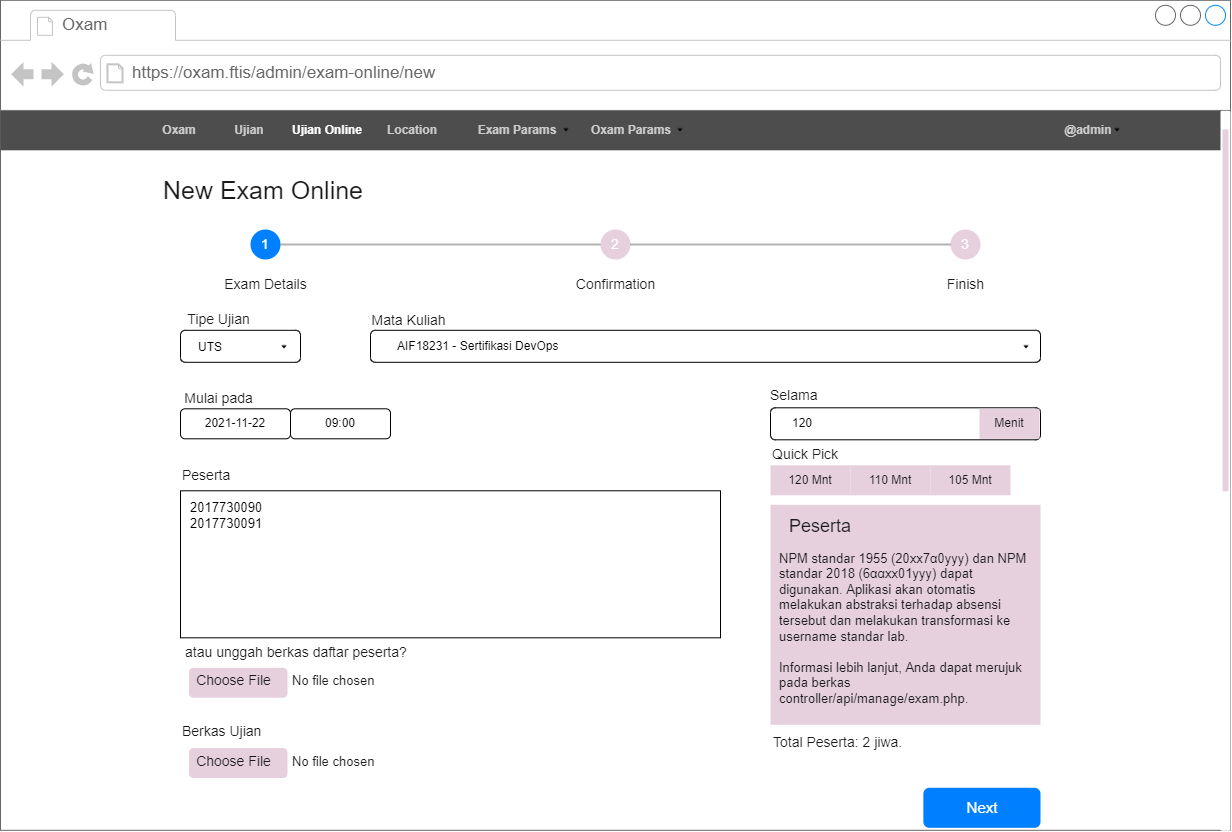
\includegraphics[width=0.8\textwidth]{images/ui designs/exam-online/manage-step-1.png}
                    \caption{Langkah pertama dalam penambahan entri ujian dengan mode otentikasi berbasis token. }
                    \label{fig:exam-online-manage-create-step1}
                \end{figure}
		        
		        Penambahan entri ujian baru pada mode ujian dengan otentikasi berbasis token terdiri dari tiga (3) tahap, yaitu tahap pengisian detail ujian (\textit{exam detail}), tahap konfirmasi (\textit{confirmation} , dan tahap penyelesaian (\textit{finsih}). Gambar \ref{fig:exam-online-manage-create-step1} merupakan tahap pertama, yaitu tahap pengisian detail dari ujian. Pada tahap ini, Tim Admin maupun Dosen yang menambahkan entri ujian dapat memilih salah satu dari tiga jenis ujian yang ada, yaitu Quiz, UTS, dan UAS. Pada bagian paling bawah (bagian ``Berkas Ujian''), Tim Admin maupun Dosen dapat menambahkan berkas ujian yang akan digunakan pada saat ujian berlangsung.   
		        
		        
		        \newpage
                \begin{figure}[H]
                    \centering
                    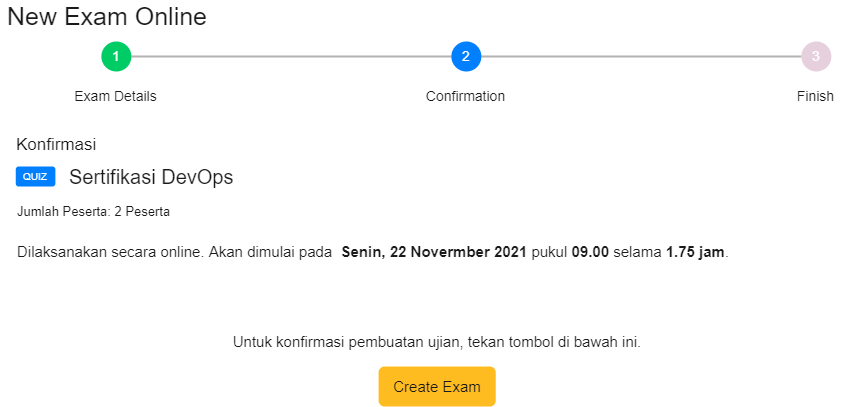
\includegraphics[width=0.85\textwidth]{images/ui designs/exam-online/manage-step-2-2.png}
                    \caption{Langkah terakhir dalam penambahan entri ujian dengan mode otentikasi berbasis token. }
                    \label{fig:exam-online-manage-create-step2}
                \end{figure}
                
                \begin{figure}[H]
                    \centering
                    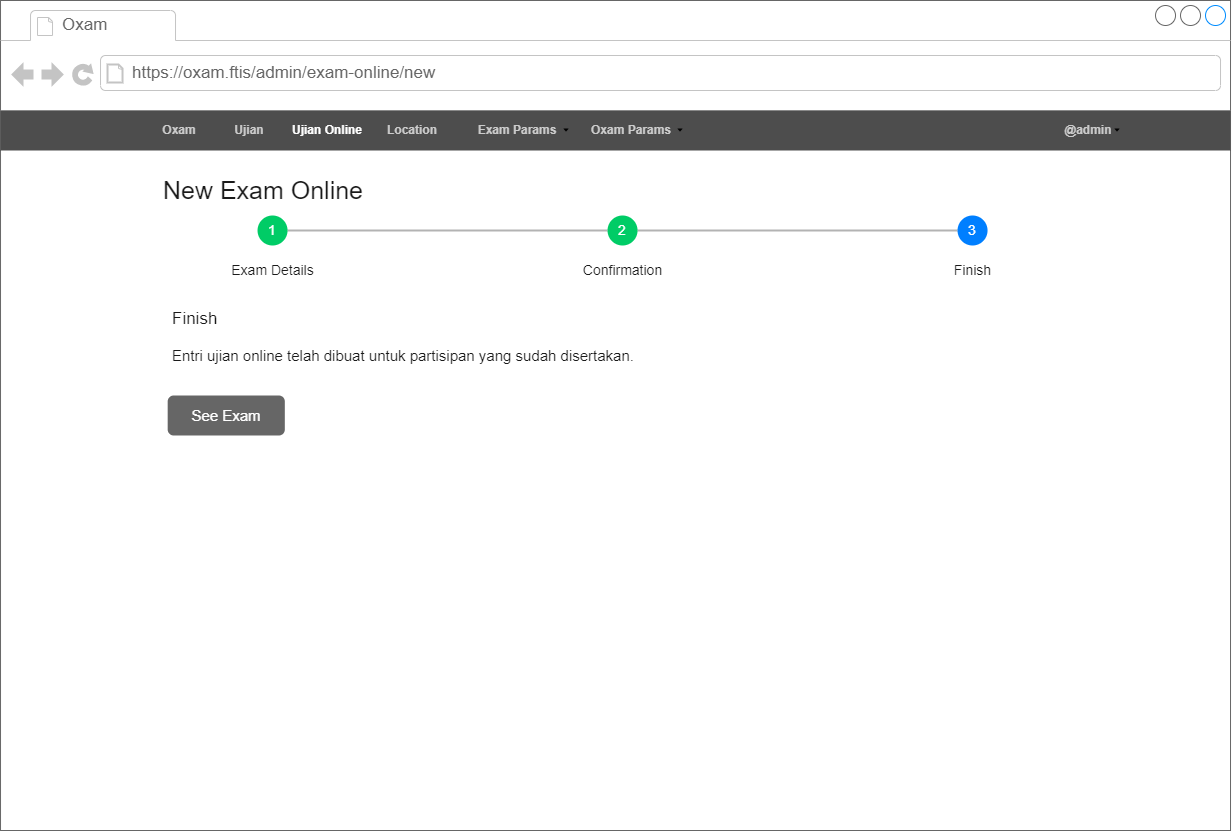
\includegraphics[width=0.85\textwidth]{images/ui designs/exam-online/manage-step-3.png}
                    \caption{Langkah kedua dalam penambahan entri ujian dengan mode otentikasi berbasis token. }
                    \label{fig:exam-online-manage-create-step3}
                \end{figure}
		        
		        Gambar \ref{fig:exam-online-manage-create-step2} merupakan tahap kedua atau tahap konfirmasi. Setelah konfirmasi selesai dilakukan dan tombol ``\textit{Create Exam}'' ditekan, maka entri ujian akan ditambahkan ke basis data dan akan menampilkan halaman penyelesaian yang dapat dilihat pada Gambar \ref{fig:exam-online-manage-create-step2}.
		        
		    \end{itemize}
		\end{itemize}
		

		\item \textbf{Melaporkan hasil penelitian dalam bentuk dokumen skripsi.}\\
		{\bf Status :} Ada sejak rencana kerja skripsi.\\
		{\bf Hasil :} -
		
		
\begin{comment}
	\item \textbf{Mengimplementasikan keseluruhan algoritma dan struktur data yang dirancang, dengan menggunakan framework OpenSteer} \\
		{\bf Status :} Ada sejak rencana kerja skripsi.\\
		{\bf Hasil :}

		\item \textbf{Melakukan pengujian (dan eksperimen) yang melibatkan responde untuk menilai hasil simulasi secara kualitatif}\\
		{\bf Status :} Ada sejak rencana kerja skripsi.\\
		{\bf Hasil :}

		\item \textbf{Menulis dokumen skripsi}\\
		{\bf Status :} Ada sejak rencana kerja skripsi.\\
		{\bf Hasil :} \lipsum[1]
		
		\item \textbf{Mempelajari cara menggunakan fitur manipulasi obstacle yang disediakan oleh framework Opensteer versi terbaru}\\
		{\bf Status :} baru ditambahkan pada semester ini\\
		{\bf Hasil :} baru direncanakan karena framework Opensteer versi paling akhir baru selesai diinstall dan dilihat-lihat bagian contoh-contoh simulasinya
\end{comment}
	
	\end{enumerate}
	
\newpage
\section{Pencapaian Rencana Kerja}
Langkah-langkah kerja yang berhasil diselesaikan dalam Skripsi 1 ini adalah sebagai berikut:
\begin{enumerate}
\item Mempelajari cara kerja OXAM dan skripsi dari Gunawan Christianto (2016730011).
\item Mempelajari React.js sebagai \textit{library front-end}.
\item Mempelajari FatFree sebagai \textit{framework} yang digunakan untuk \textit{back-end}.
\end{enumerate}


\begin{comment}
\section{Kendala yang Dihadapi}
%TULISKAN BAGIAN INI JIKA DOKUMEN ANDA TIPE A ATAU C
Kendala - kendala yang dihadapi selama mengerjakan skripsi :
\begin{itemize}
	\item Terlalu banyak melakukan prokratinasi
	\item Terlalu banyak godaan berupa hiburan (game, film, dll)
	\item Skripsi diambil bersamaan dengan kuliah ASD karena selama 5 semester pertama kuliah tersebut sangat dihindari dan tidak diambil, dan selama 4 semester terakhir kuliah tersebut selalu mendapat nilai E
	\item Mengalami kesulitan pada saat sudah mulai membuat program komputer karena selama ini selalu dibantu teman
\end{itemize}
\end{comment}

\vspace{1cm}
\centering Bandung, \tanggal\\
\vspace{2cm} \nama \\ 
\vspace{1cm}

Menyetujui, \\
\ifdefstring{\jumpemb}{2}{
\vspace{1.5cm}
\begin{centering} Menyetujui,\\ \end{centering} \vspace{0.75cm}
\begin{minipage}[b]{0.45\linewidth}
% \centering Bandung, \makebox[0.5cm]{\hrulefill}/\makebox[0.5cm]{\hrulefill}/2013 \\
\vspace{2cm} Nama: \pembA \\ Pembimbing Utama
\end{minipage} \hspace{0.5cm}
\begin{minipage}[b]{0.45\linewidth}
% \centering Bandung, \makebox[0.5cm]{\hrulefill}/\makebox[0.5cm]{\hrulefill}/2013\\
\vspace{2cm} Nama: \pembB \\ Pembimbing Pendamping
\end{minipage}
\vspace{0.5cm}
}{
% \centering Bandung, \makebox[0.5cm]{\hrulefill}/\makebox[0.5cm]{\hrulefill}/2013\\
\vspace{2cm} Nama: \pembA \\ Pembimbing Tunggal
}
\end{document}

